% !TeX spellcheck = sr_SR-Serbian
% Format teze zasnovan je na paketu memoir
% http://tug.ctan.org/macros/latex/contrib/memoir/memman.pdf ili
% http://texdoc.net/texmf-dist/doc/latex/memoir/memman.pdf
% 
% Prilikom zadavanja klase memoir, navedenim opcijama se podešava 
% veličina slova (12pt) i jednostrano štampanje (oneside).
% Ove parametre možete menjati samo ako pravite nezvanične verzije
% mastera za privatnu upotrebu (na primer, u b5 varijanti ima smisla 
% smanjiti 

\documentclass[12pt,oneside]{memoir}

% Paket koji definiše sve specifičnosti mastera Matematičkog fakulteta
\usepackage{matfmaster}
%
% Podrazumevano pismo je ćirilica.
%   Ako koristite pdflatex, a ne xetex, sav latinički tekst na srpskom jeziku
%   treba biti okružen sa \lat{...} ili \begin{latinica}...\end{latinica}.
%
% Opicija [latinica]:
%   ako želite da pišete latiniciom, dodajte opciju "latinica" tj.
%   prethodni paket uključite pomoću: \usepackage[latinica]{matfmaster}.
%   Ako koristite pdflatex, a ne xetex, sav ćirilički tekst treba biti
%   okružen sa \cir{...} ili \begin{cirilica}...\end{cirilica}.
%
% Opcija [biblatex]:
%   ako želite da koristite reference na više jezika i umesto paketa
%   bibtex da koristite BibLaTeX/Biber, dodajte opciju "biblatex" tj.
%   prethodni paket uključite pomoću: \usepackage[biblatex]{matfmaster}
%
% Opcija [b5paper]:
%   ako želite da napravite verziju teze u manjem (b5) formatu, navedite
%   opciju "b5paper", tj. prethodni paket uključite pomoću: 
%   \usepackage[b5paper]{matfmaster}. Tada ima smisla razmisliti o promeni
%   veličine slova (izmenom opcije 12pt na 11pt u \documentclass{memoir}).
%
% Naravno, opcije je moguće kombinovati.
% Npr. \usepackage[b5paper,biblatex]{matfmaster}

% Pomoćni paket koji generiše nasumičan tekst u kojem se javljaju sva slova
% azbuke (nema potrebe koristiti ovo u pravim disertacijama)
\usepackage{pangrami}

% Paket koji obezbeđuje ispravni prikaz ćiriličkih italik slova kada
% se koristi pdflatex. Zakomentarisati ako na sistemu koji koristite ovaj
% paket nije dostupan ili ako ne radi ispravno.
\usepackage{cmsrb}
\usepackage{minted2}
\setminted{fontsize=\small}


\usepackage{amsthm}
\newtheorem{exmp}{Пример}

% Ostali paketi koji se koriste u dokumentu
%\usepackage{listings} % listing programskog koda

% Datoteka sa literaturom u BibTex tj. BibLaTeX/Biber formatu
\bib{implementacija_tekst_editora_za_pisanje_koda}

% Ime kandidata na srpskom jeziku (u odabranom pismu)
\autor{Бојан Барџић}
% Naslov teze na srpskom jeziku (u odabranom pismu)
\naslov{Имплементација текст едитора за писање кода}
% Godina u kojoj je teza predana komisiji
\godina{2025}
% Ime i afilijacija mentora (u odabranom pismu)
\mentor{др Весна \textsc{Маринковић}, доцент\\ Универзитет у Београду, Математички факултет}
% Ime i afilijacija prvog člana komisije (u odabranom pismu)
\komisijaA{др Милан \textsc{Банковић}, доцент \\ Универзитет у Београду, Математички факултет}
% Ime i afilijacija drugog člana komisije (u odabranom pismu)
\komisijaB{др Иван \textsc{Чукић}, доцент\\ Универзитет у Београду, Математички факултет}
% Ime i afilijacija trećeg člana komisije (opciono)
% \komisijaC{}
% Ime i afilijacija četvrtog člana komisije (opciono)
% \komisijaD{}
% Datum odbrane (obrisati ili iskomentarisati narednu liniju ako datum odbrane nije poznat)
\datumodbrane{15. јануар 2016.}

% Apstrakt na srpskom jeziku (u odabranom pismu)
\apstr{%
\pangrami
}

% Ključne reči na srpskom jeziku (u odabranom pismu)
\kljucnereci{}


\begin{document}
% ==============================================================================
% Uvodni deo teze
\frontmatter
% ==============================================================================
% Naslovna strana
\naslovna
% Strana sa podacima o mentoru i članovima komisije
\komisija
% Strana sa posvetom (u odabranom pismu)
\posveta{}
% Strana sa podacima o disertaciji na srpskom jeziku
\apstrakt
% Sadržaj teze
\tableofcontents*

% ==============================================================================
% Glavni deo teze
\mainmatter
% ==============================================================================

% ------------------------------------------------------------------------------
\chapter{Увод}
% ------------------------------------------------------------------------------

\section{Текст едитори}

\paragraph{}
\emph{Текст едитор} је програм за креирање, мењање, измену и прегледање текстуалних датотека. Најчешћи типови датотека
који се обрађују у текст едиторима су једноставне текстуалне датотеке, 
датотеке које садржe изворни код, код језика за означавање као и конфигурационе датотеке.  Неки од најпознатијих текст еидотра су \begin{latinica}\textit{Visual Studio Code}
\end{latinica} \cite{VSC}, \begin{latinica}\textit{Notepad}\end{latinica} \cite{Notepad},
\begin{latinica}\textit{Notepad++}\end{latinica} \cite{Notepad++}, \begin{latinica}\textit{VIM}
\end{latinica} \cite{VIM} и \begin{latinica}\textit{Emacs}\end{latinica} \cite{Emacs}.

\paragraph{}
Постоји више врста текст едитора. Постоје едитори \emph{једноставног текста}
(енг. \begin{latinica}\textit{plain text}\end{latinica}), где информација
о датотеци представља само текст. Поред њих, постоје и едитори \emph{богатог текста}
(енг. \begin{latinica}\textit{rich text}\end{latinica}), где информација о датотеци
поред текста садржи и неке додатне информације везано за изглед текста (фонт, величина слова, боја, маргине). Овај рад ће се бавити искључиво
едиторима једноставног текста.

\paragraph{}
Ранији текст едитори били су приказивани у преко стандардног излаза \emph{терминала}, 
пример једног оваквог едитора је \begin{latinica}\textit{VIM}\end{latinica} \cite{VIM}. 
Тек касније се јављају едитори са \emph{графичким корисничким окружењем} 
(енг. \begin{latinica}\textit{graphical user interface}\end{latinica}). Први
такви едитори углавном су се састојали од \emph{поља за уређивање} 
(енг. \begin{latinica}\textit{editing area}\end{latinica}), на ком је
приказан садржај отворене датотеке коју корисник уређује. Поље за уређивање
представља главну компоненту сваког едитора. 

\paragraph{}
Поред тога, једне од основних компоненти
корисничког окружења су \emph{мени} (енг. \begin{latinica}\textit{menu}\end{latinica}) и
\emph{статусна линија} (енг. \begin{latinica}\textit{status bar}\end{latinica}). 
Мени се обично налази испод насловне линије и преко њега се приступа разним
функционалностима које текст едитор нуди коирснику као што су манипулација датотекама,
операције са \emph{привременом меморијом} 
(енг. \begin{latinica}\textit{clipboard}\end{latinica}),
претрага итд. Статусна линија се налази на дну текст едитора и на њој су исписане
информације као што су име отворене датотеке, положај \emph{курсора}, енкодирање итд.

\paragraph{}
Временом се развојем текст едитора намењеним специфично за писање програмског кода
корисничко окружење проширује додатним компонентама као што су терминал, претраживач
датотека итд. На слици \ref{fig:layout} илустрован распоред ових
компоненти на једном текст едитору за писање кода.

\begin{figure}[!ht]
	\centering
	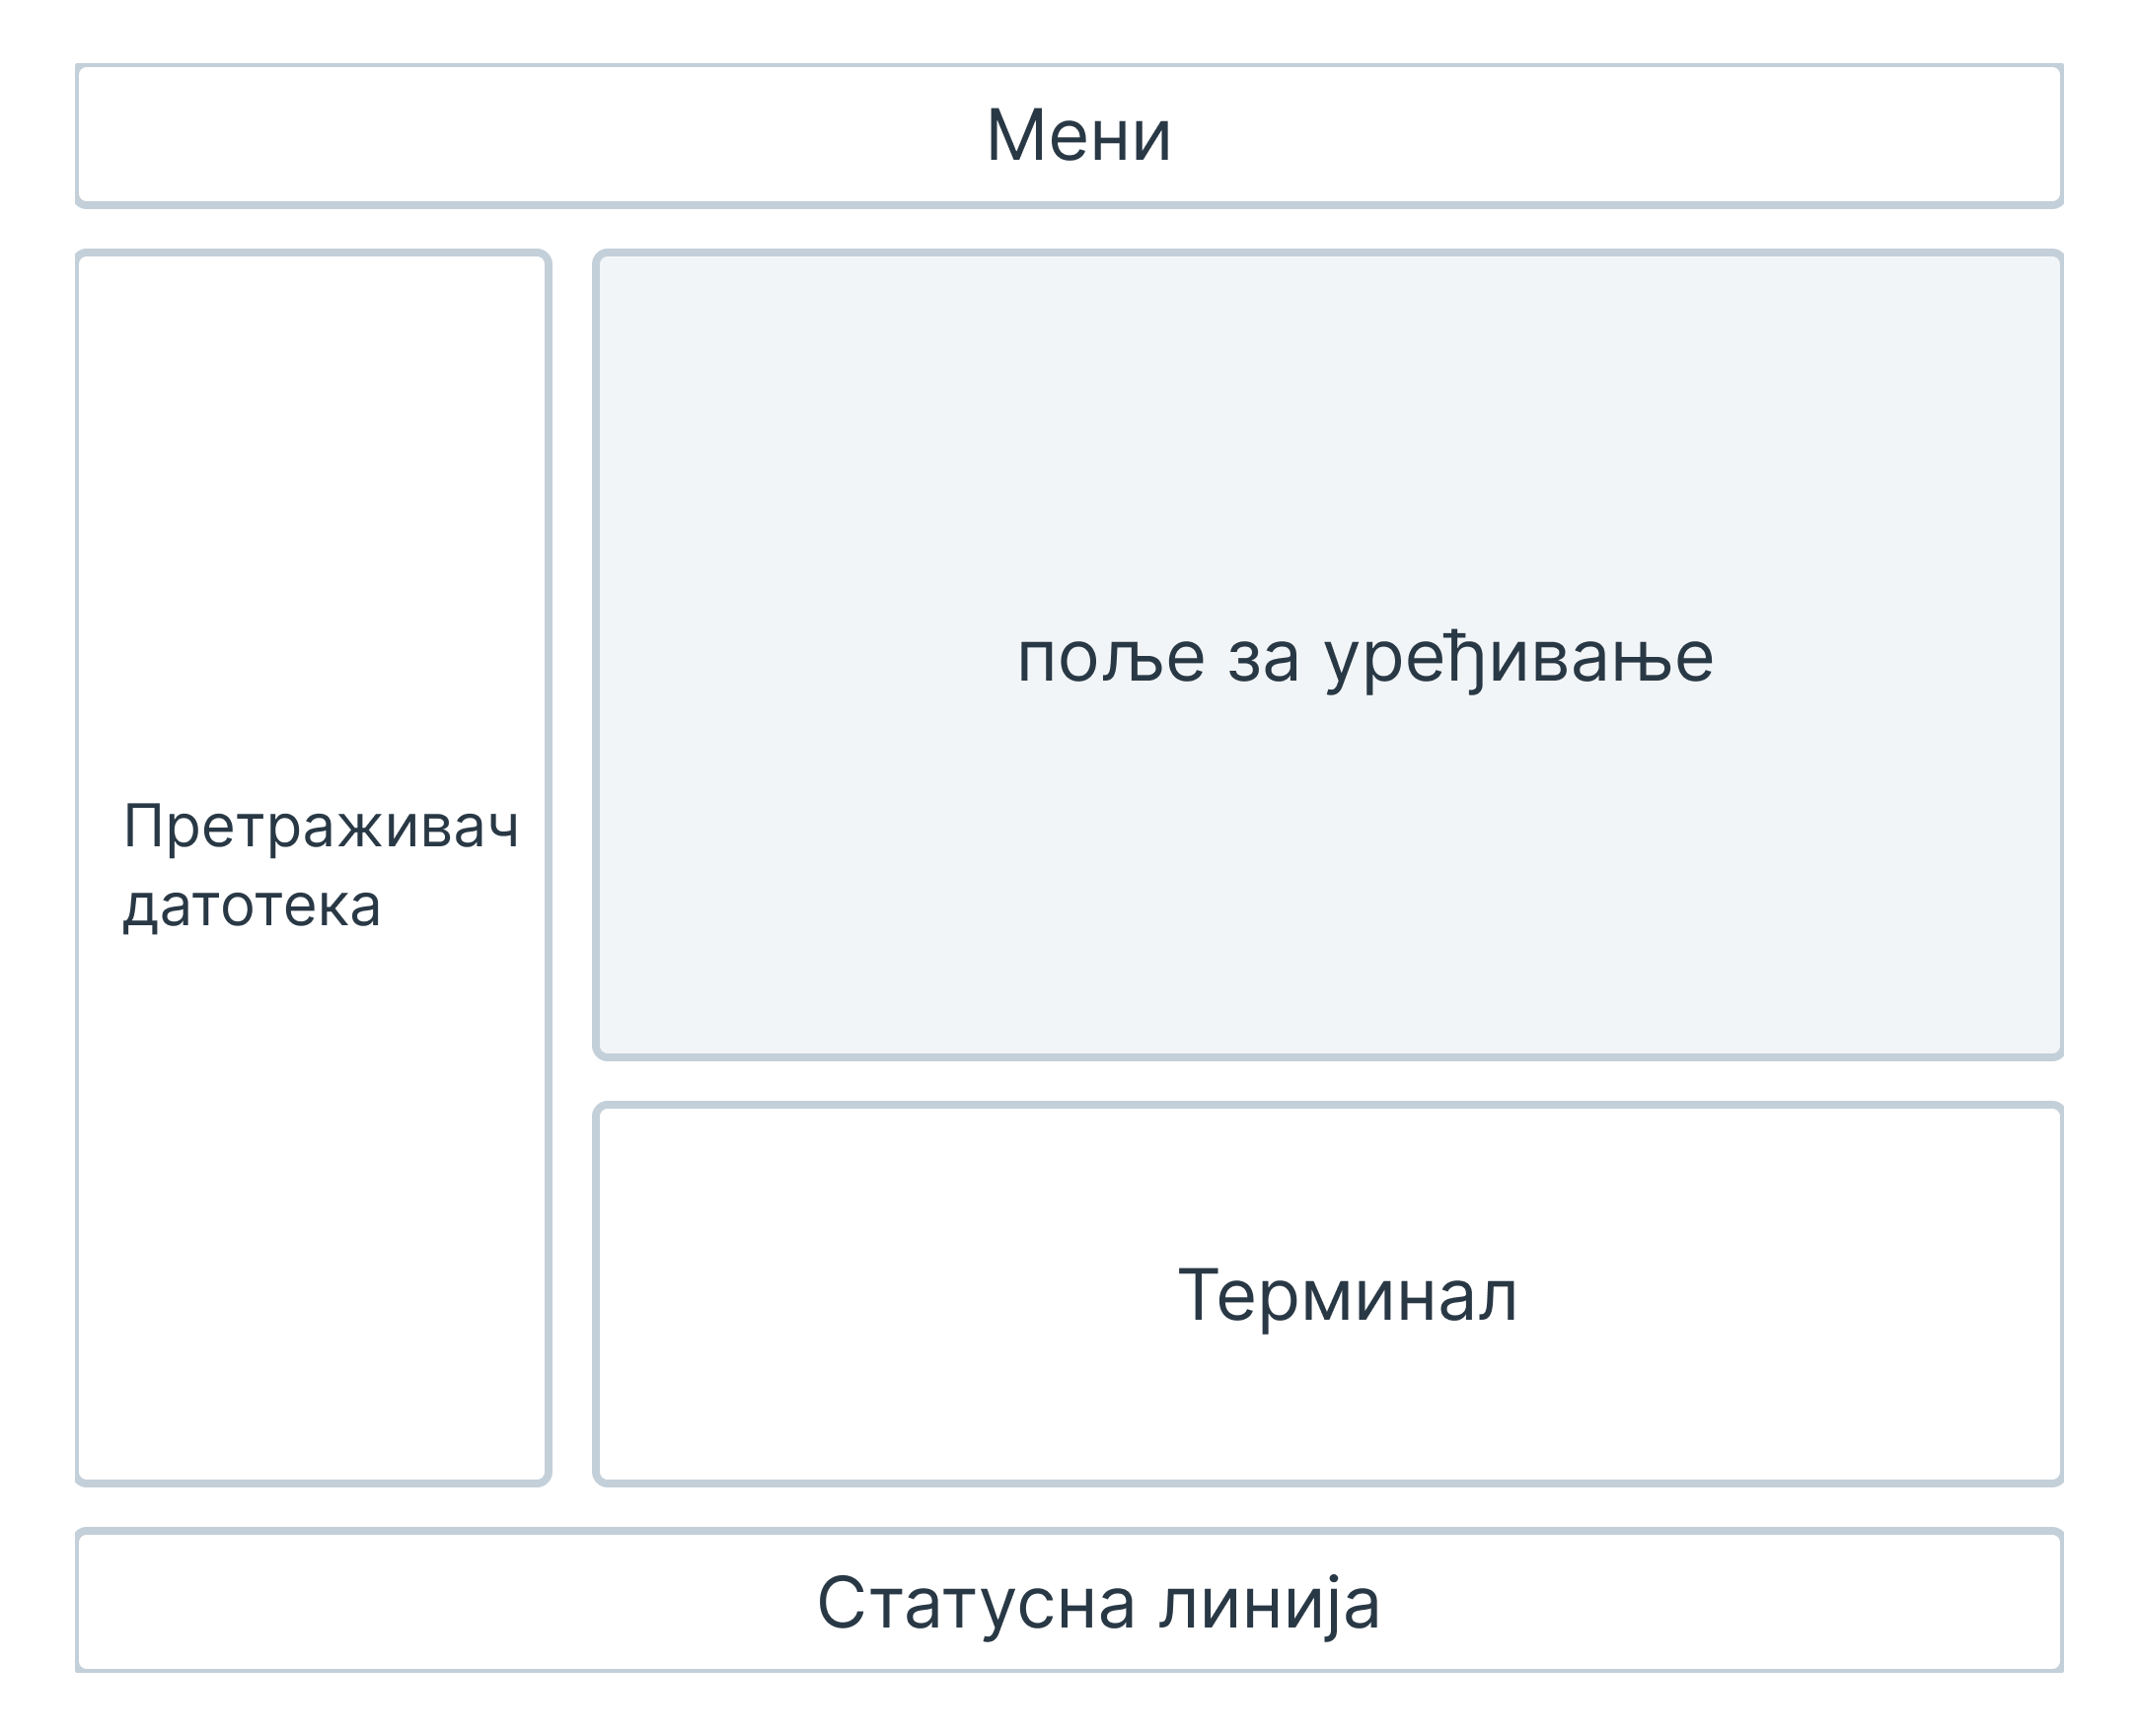
\includegraphics[width=0.8\textwidth]{images/raspored.png}
	\caption{Распоред компоненти текст едитора за писање кода}
	\label{fig:layout}
\end{figure}

\paragraph{}
Неке од основних функционалности које сваки едитор треба да нуди су креирање, отварање
и измена датотека, oперације са привременом меморијом, претрага, поништавање и 
понављање. Временом су неке од напреднијих функционалности у текст едиторима
за писање кода, као што су назначавање кода и аутомаско комплетирање текста као и
функционалности везане за изглед еидтора (тема, избор фонта, подешавање величине слова)
постале подразумеване од стране корисника.

\paragraph{}
Када се говори о текст едиторима за писање кода, развој додатних напредних фукционалности
довео је до појаве великог броја различитих текст едитора. Сваки од њих нудећи како
одређени скуп истих функционалности, тако и напредне функционалности специфичне за тај
едитор. Такође је сваки едитор имао своје корисничко окружење различито од осталих. Сваки од нових едитора имао је за циљ да унапреди искуство писања кода у односу на популарне
текст едиторе у то време на основу својих иновација. Због различитих преференци корисника
при писању кода и при избору корисничког интерфејса данас постоји разноврстан скуп
популарних текст едитора.

\paragraph{}
У данашње време текст едитори имају велики значај у разним областима.
Осим што су неизоставни део алата које користе програмери, нудећи својим
функционалностима удобније и брже писање кода, преко пословне употребе ради
писања докумената, па све до образовања и писања научних радова. Изузетно је ретко пронаћи корисника који ниједном током рада на рачунару није
имао потребу за текст едитором.

\paragraph{}
Корисници у данашње време често узимају едиторе текста за готово. Сматра се основним 
програмом који постоји на сваком рачунару. Зато је при овом раду имплементиран нови
едитор текста под именом \emph{ЈЕТ} (једноставан едитор текста) да би се прошло кроз имплементацију свих детаља потребних за израду 
једног едитора текста и стекло боље разумевање шта се дешава "испод хаубе" програма
који се свакодневно употребљава од стране корисника као и имплементација неких 
нестандардних функционалности који могу бити корисне при писању кода.

\chapter{Структуре података у текст едиторима}
\paragraph{}
Уколико постоји низ карактера дужине \(n\), основне операције измене над њим су 
уметање неког низа карактера на неки индекс или брисање неког подниза карактера из њега.
Пошто се текст у датотеци се може посматрати као линеарни низ карактера, све измене које
се врше над текстуалном датотеком се могу посматрати на овај начин. 
Када би комплетан садржај текстуалне датотеке која је отворена био чуван као јединствен
низ карактера, операције уметања и брисања текста биле би временски јако скупе (реда
\(O(n)\), где је \(n\) дужина текста) и њихово узастопно извршавање над неким дугачким
текстом би имало за последицу изузетну неефикасност текст едитора. Како би се овај 
проблем превазишао осмишљене су различите структуре података које ове операције
врше ефикасније. Најпознатије међу њима су \emph{бафер са размацима}
(енг. \begin{latinica}\textit{gap buffer}\end{latinica}), \emph{уже} (енг. 
\begin{latinica}\textit{rope}\end{latinica}) и \emph{табела делова} (енг. 
\begin{latinica}\textit{piece table}\end{latinica}).

\section{Бафер са размацима}
\paragraph{}
Бафер са размацима представља одређени вид проширења низа карактера који омогућава
ефикасније операције уметања и брисања у ситуацији када се измене врше на блиским
локацијама у тексту. Структура се заснива на идеји да постоји један линеаран низ чија је средина "празна", док се са леве и десне стране налази текст.
Како се врше измене над неким делом текста тако се средина "помера" превлачењем последњег елемента леве стране на почетак десне или обрнуто. Када се бафер попуни (размак није довољно велики за нову операцију), тада се алоцира нови бафер већих димензија, најчешће двоструко веће димензије, и у њега се копира текст из старог бафера.

\paragraph{}
У односу на класичан низ карактера, бафер са размацима је временски доста 
ефикаснији јер не захтева реалокацију низа при свакој измени. Ефикасност операција уметања и брисања зависи највише од тога колики је размак између индекса на коме се  
врши измена текста и леве или десне границе размака. Ако је размак већ на потребној позицији, временска сложеност је \(O(1)\). Међутим, ако је размак на једном крају а
потребно је да се мења други крај текста сложеност ће бити \(O(n)\). У просечном случају
временска сложеност наведених операција је константна, јер се карактери најчешће пишу (и бришу) један за другим. Треба напоменути и то да је с времена на време потребно вршити
реалокацију низа, која је линеарне сложености у односу на дужину текста.

\paragraph{}
Разматрана структура података је једноставна за имплементацију и чест је избор
при иплементацији текст едиотра. Познати текст едитори \begin{latinica}\textit{Emacs}\end{latinica} \cite{Emacs} и 
\begin{latinica}\textit{Notepad++}\end{latinica} \cite{Notepad++}
користe ову структуру у својој имплементацији.

\begin{figure}[!ht]
	\centering
	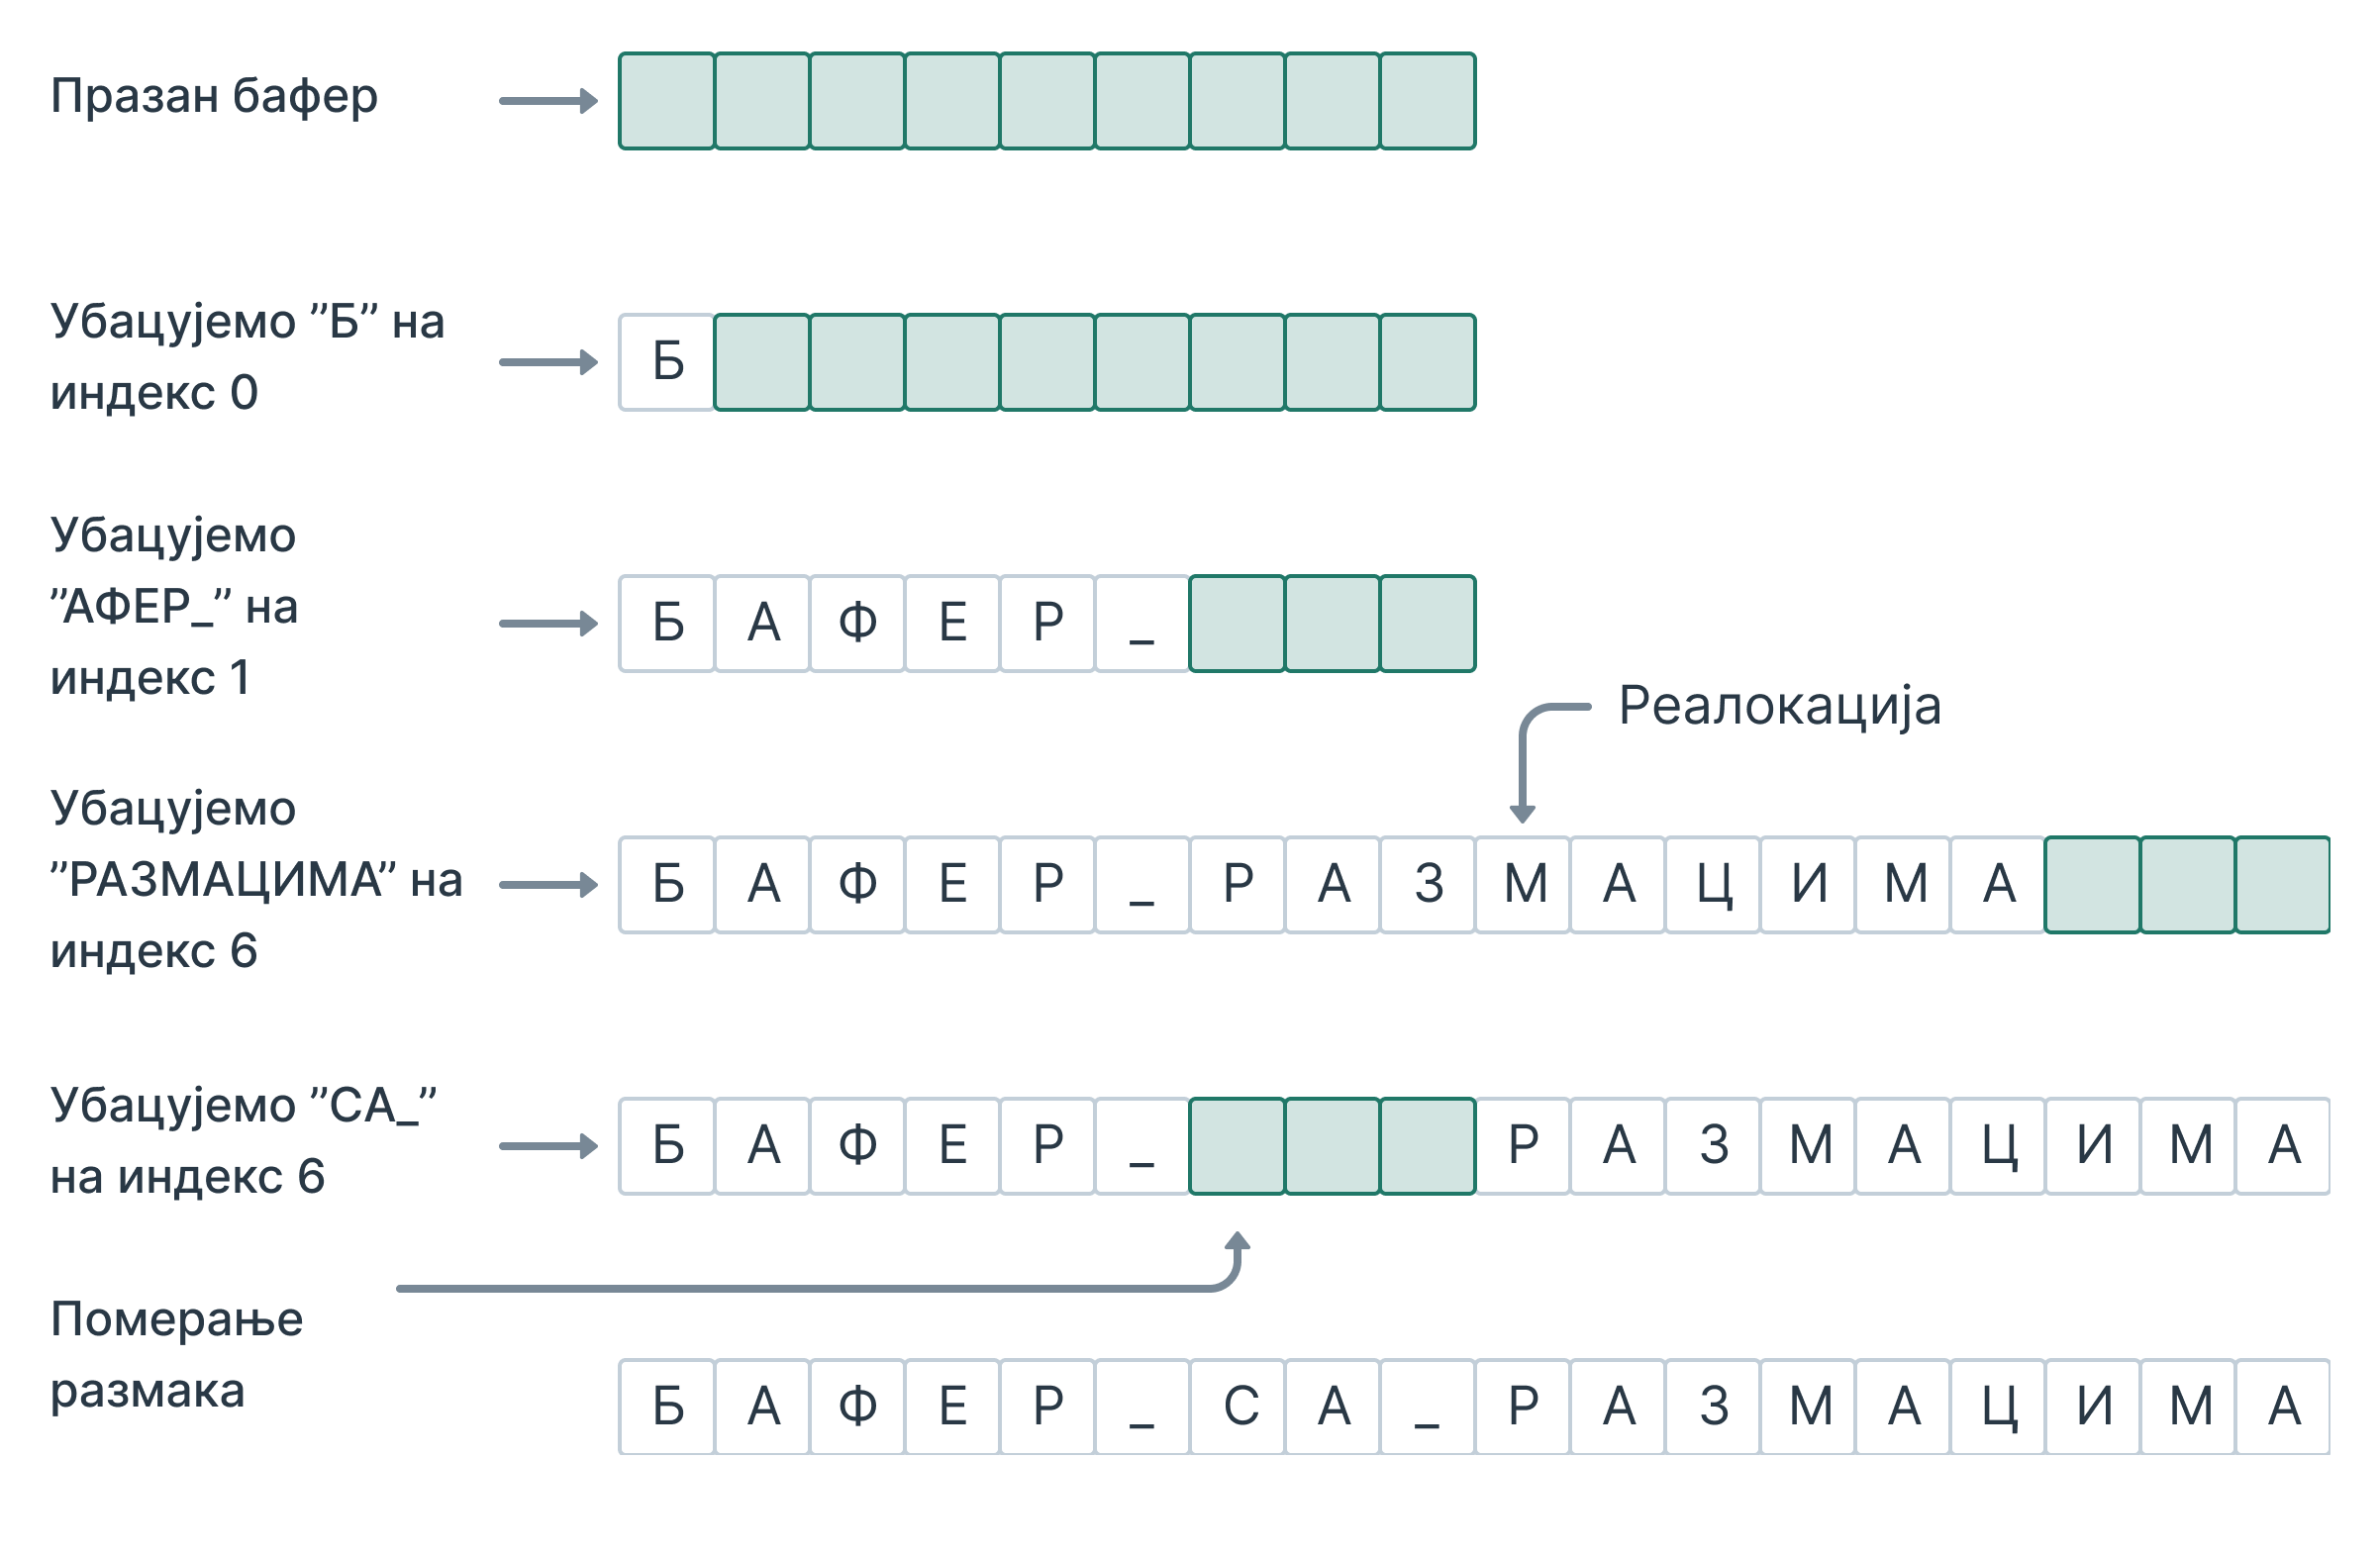
\includegraphics[width=1.1\textwidth]{images/Bafer_3.png}
	\caption{Илустрација бафера са размаком}
	\label{fig:gap_buffer}
\end{figure}

\begin{exmp}

На слици \ref{fig:gap_buffer} приказана је  илустрација рада бафера са размаком.
У првом кораку бафер је празан. У следећем кораку се додаје ниска \textit{"б"} на почетну позицију. После тога на крај текста се додаје ниска \textit{"афер\_"}, а после тога и ниска
\textit{"размацима"}.  Пошто је бафер у том тренутку пун, врши се реалокација. Када се текст прекопира у нови низ, помера се почетак празног дела на жељени индекс и додаје се
нова ниска. У последњем кораку се додаје ниска \textit{"са\_"} на индекс број 6. 

\end{exmp}


\section{Уже}
\paragraph{}
Уже је бинарно стабло у коме сви чворови који нису листови садрже број карактера у 
левом подстаблу тог чвора. У листовима се налазе ниске које садрже делове текста. 
Када се прође кроз листове редом од првог листа слева до крајњег десног листа, 
добија се целокупан текст.

\paragraph{}
Предност ове структуре у односу на обичан низ карактера је што операције као што су уметање, брисање и претрага текста у просечном случају имају временску сложеност \(O(\log{}n)\) (где је \(n\) дужина текста), а не \(O(n)\). Такође, није потребно чувати
текст у непрекидном делу меморије, већ делови текста могу бити разбацани по меморији.

\paragraph{}
Мане ужета јесу што је то комплексна структура и чешће су грешке како у раду са њом,
тако и при њеној имплементацији. Поред тога, заузима више меморије него обичан низ
карактера (због потребе за чувањем унутрашњих чворова стабла). Пример текст едитора који
користи уже у својој имплементацији је \begin{latinica}\textit{Xi}\end{latinica} \cite{Xi}.
На слици \ref{fig:rope_example} приказан је пример ужета који садржи текст 
\textit{"Ово је пример ужета"}.

\begin{figure}[!ht]
	\centering
	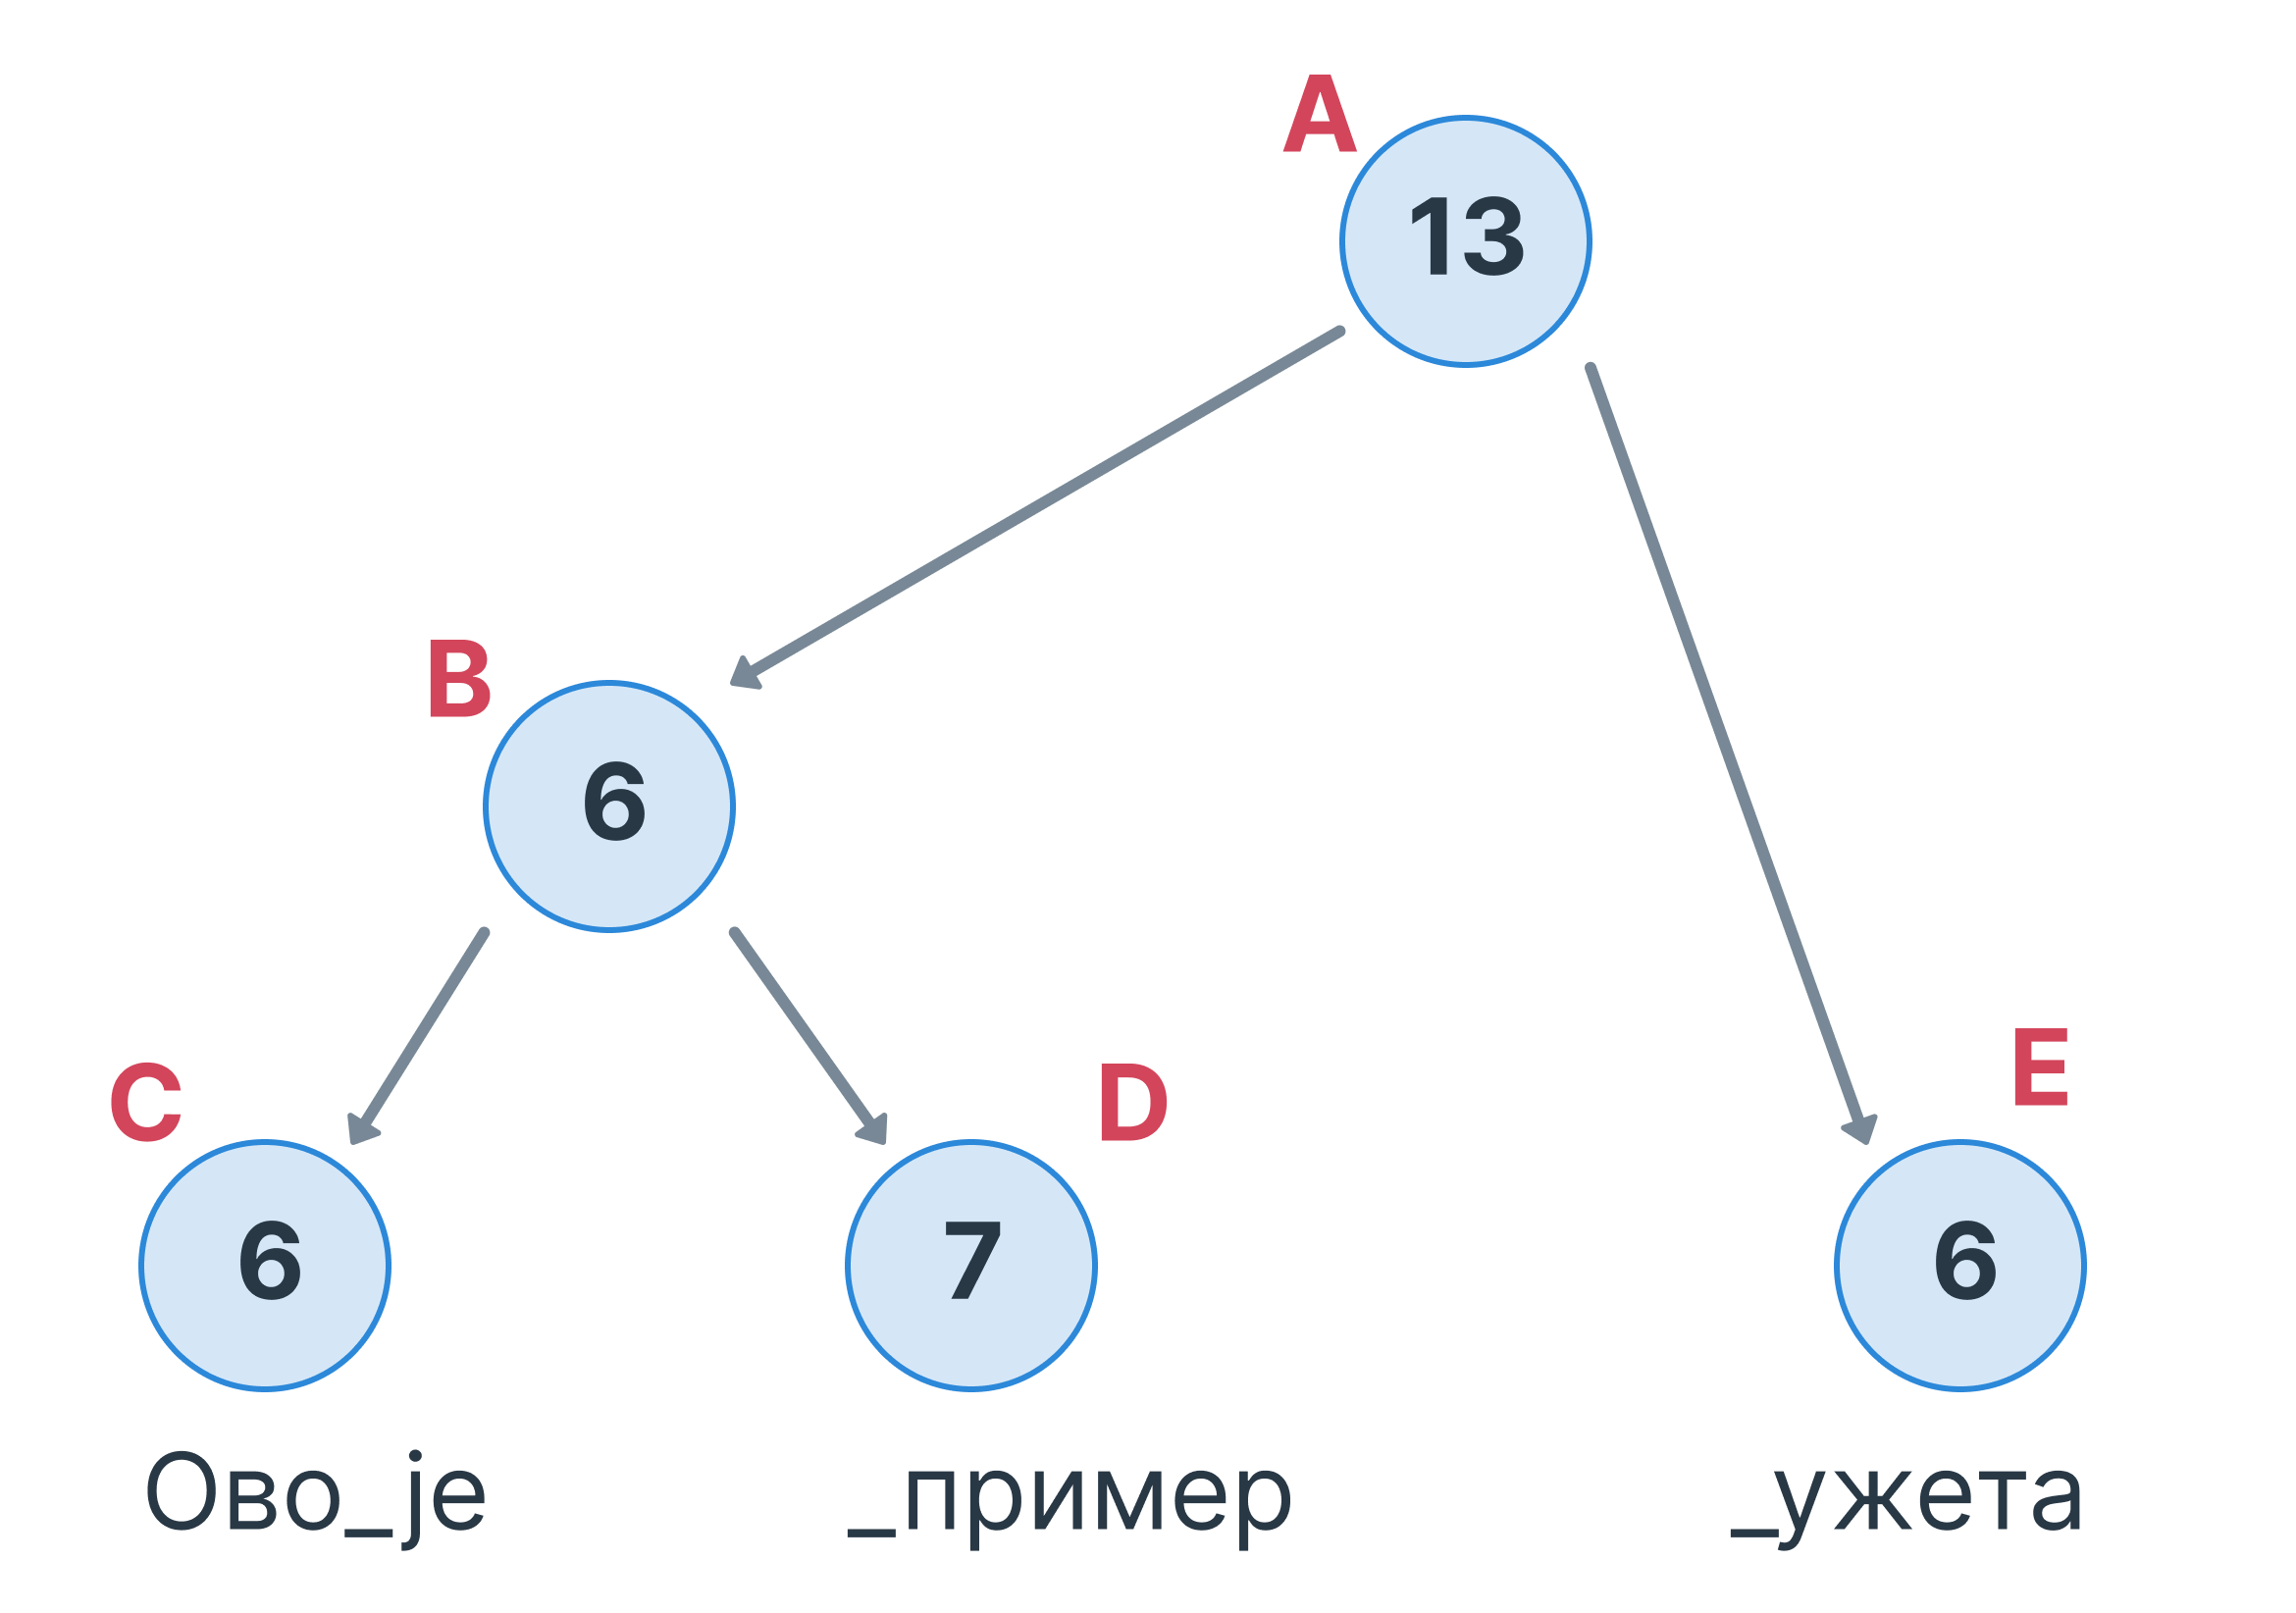
\includegraphics[width=0.7\textwidth]{images/rope_example.png}
	\caption{Пример једног ужета}
	\label{fig:rope_example}
\end{figure}

\subsection{Претрага}
\paragraph{}
Приступ карактеру на \(i\)-том  индексу се врши тако што се рекурзивно пролази кроз стабло 
почевши од корена. Ако је индекс мањи од вредности у текућем чвору, настављамо претрагу у његовом левом подстаблу. У супротном од \(i\) се одузима вредност коју чува тренутни 
чвор и наставља се претрага у његовом десном подстаблу. Када се наиђе на лист враћа се
\(i\)-ти карактер из ниске која се налази у чвору. Сложеност операције је иста као код
претраге бинарног стабла, а то је \(O(\log{}n)\). 

\begin{figure}
  \centering
  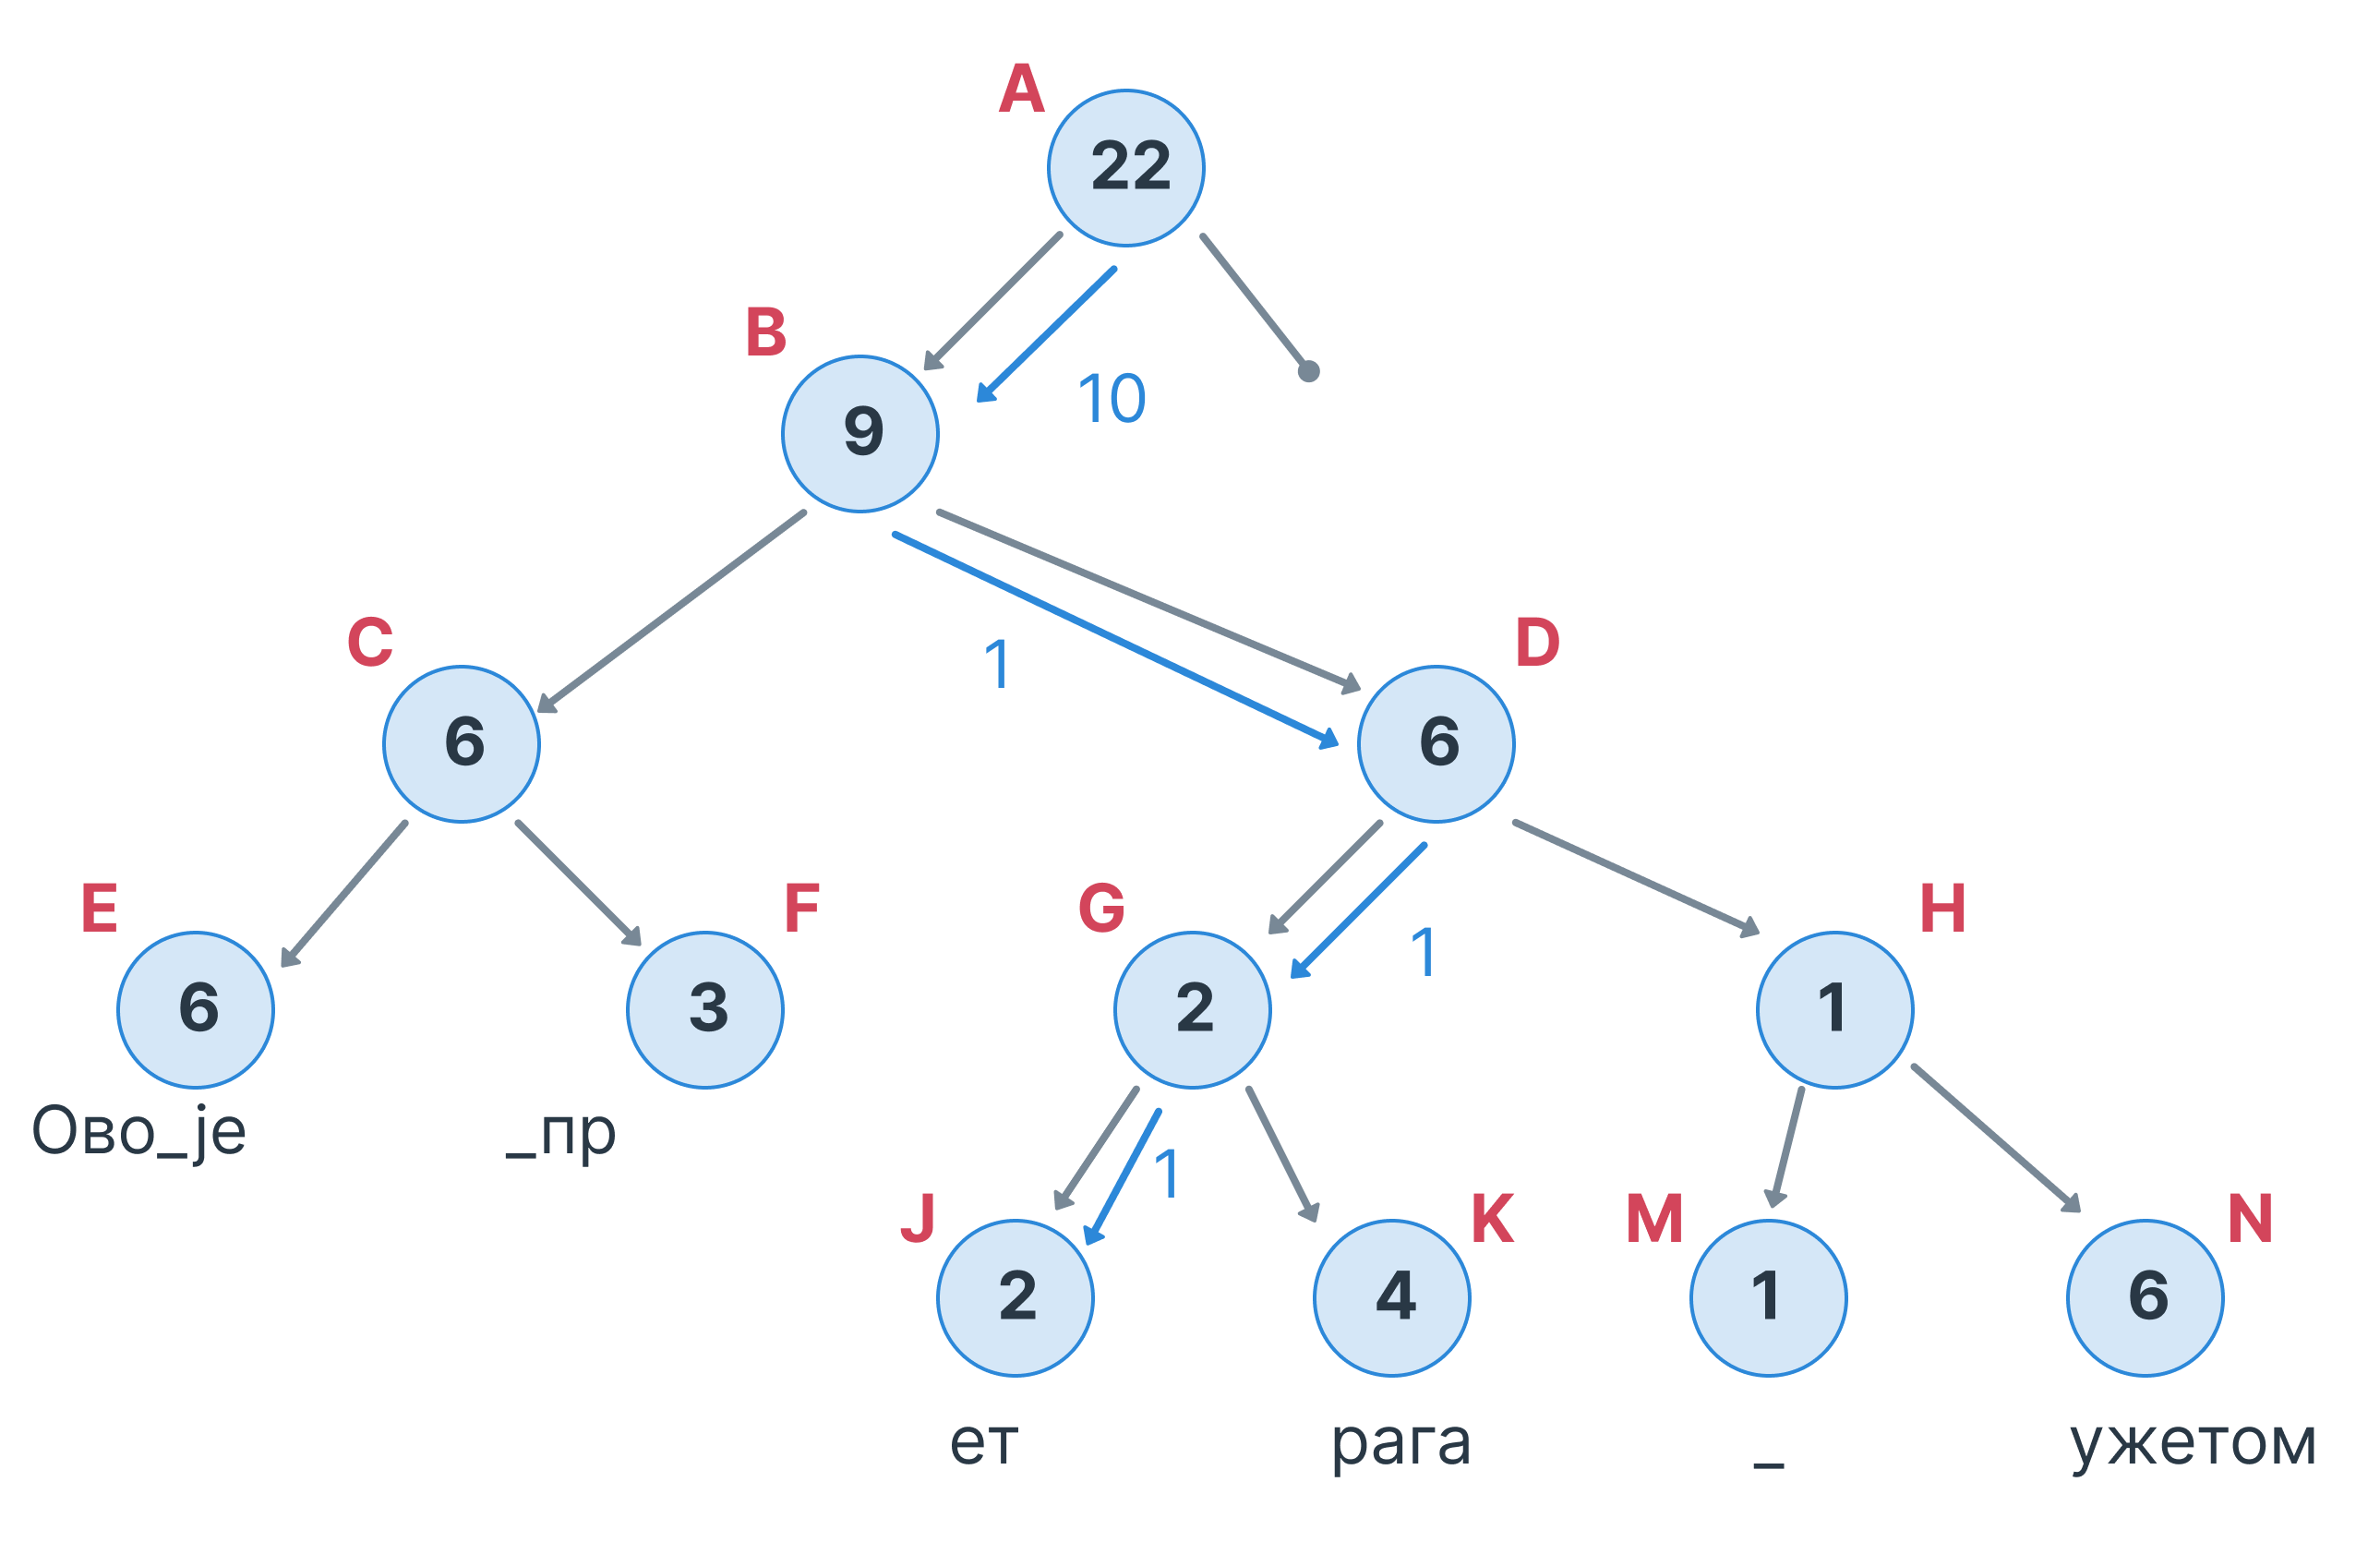
\includegraphics[width=0.8\textwidth]{images/rope_search_1.png}
  \caption{Претрага помоћу ужета}
  \label{fig:rope_search}
\end{figure}

\begin{exmp}
Пример претраге дат је на слици \ref{fig:rope_search}.
Нека је код ужета које садржи текст \textit{"Ово је претрага ужетом"} потребно дохватити карактер текста на индексу 10 тј. карактер \textit{"т"}. Прво се обилази корен 
који садржи дужину укупног текста, пошто је тражени индекс мањи од вредности у тренутном
чвору иде се у његово лево подстабло. Следећи чвор садржи вредност 9, што значи да је
тражени индекс већи од вредности. Одузима се та вредност од траженог индекса и претрага се
наставља у десном подстаблу тренутног чвора. Сада је тражени индекс 1 и он се поново
упоређује са тренутним чвором. Пошто је 1 мање од 6 прелази се у лево подстабло. 
У следећем чвору вредност је 2 па се поново иде у лево подстабло. На крају се наилази на
лист који садржи ниску \textit{"ет"} и дохвата се карактер на индексу 1 тј. \textit{"т"},
што је исправна вредност.

\end{exmp}

\paragraph{}
Пре него што буде обрађена операција брисања, прво ће бити уведене две нове операције које ће бити потребне за њену реализацију. Прва операција је надовезивање једног ужета на друго,
док је друга операција дељење једног ужета на два нова ужета по неком карактеру.


\subsection{Надовезивање}
\paragraph{}
\emph{Надовезивање} (енг. \begin{latinica}\textit{concatenation}\end{latinica}) је
операција којом се на уже, које садржи текст \(t_1\), надовезује друго уже које садржи
текст \(t_2\) и добија се ново уже које садржи текст \(t_1t_2\). Надовезивање два ужета, \(r_1\) и \(r_2\), се врши тако што се направи нови родитељски чвор чије ће лево дете бити
корен од \(r_1\), а десно корен од  \(r_2\). Вредност новог чвора ће бити сума дужина
ниски у свим листовима ужета \(r_1\). Да би се израчунала вредност новог корена потребно је
израчунати суму дужина ниски свих листова који се налазе у \(r_1\). То се постиже
рекурзивним обиласком \(r_1\), где се на коначну суму додаје вредност тренутног чвора и
затим се рекурзивно обилази десно подстабло тренутног чвора. Сложеност ове 
операције је \(O(\log{}n)\) за балансирано стабло. Пример надовезивања два 
ужета се може видети на слици \ref{fig:rope_concat}

\begin{figure}
  \centering
  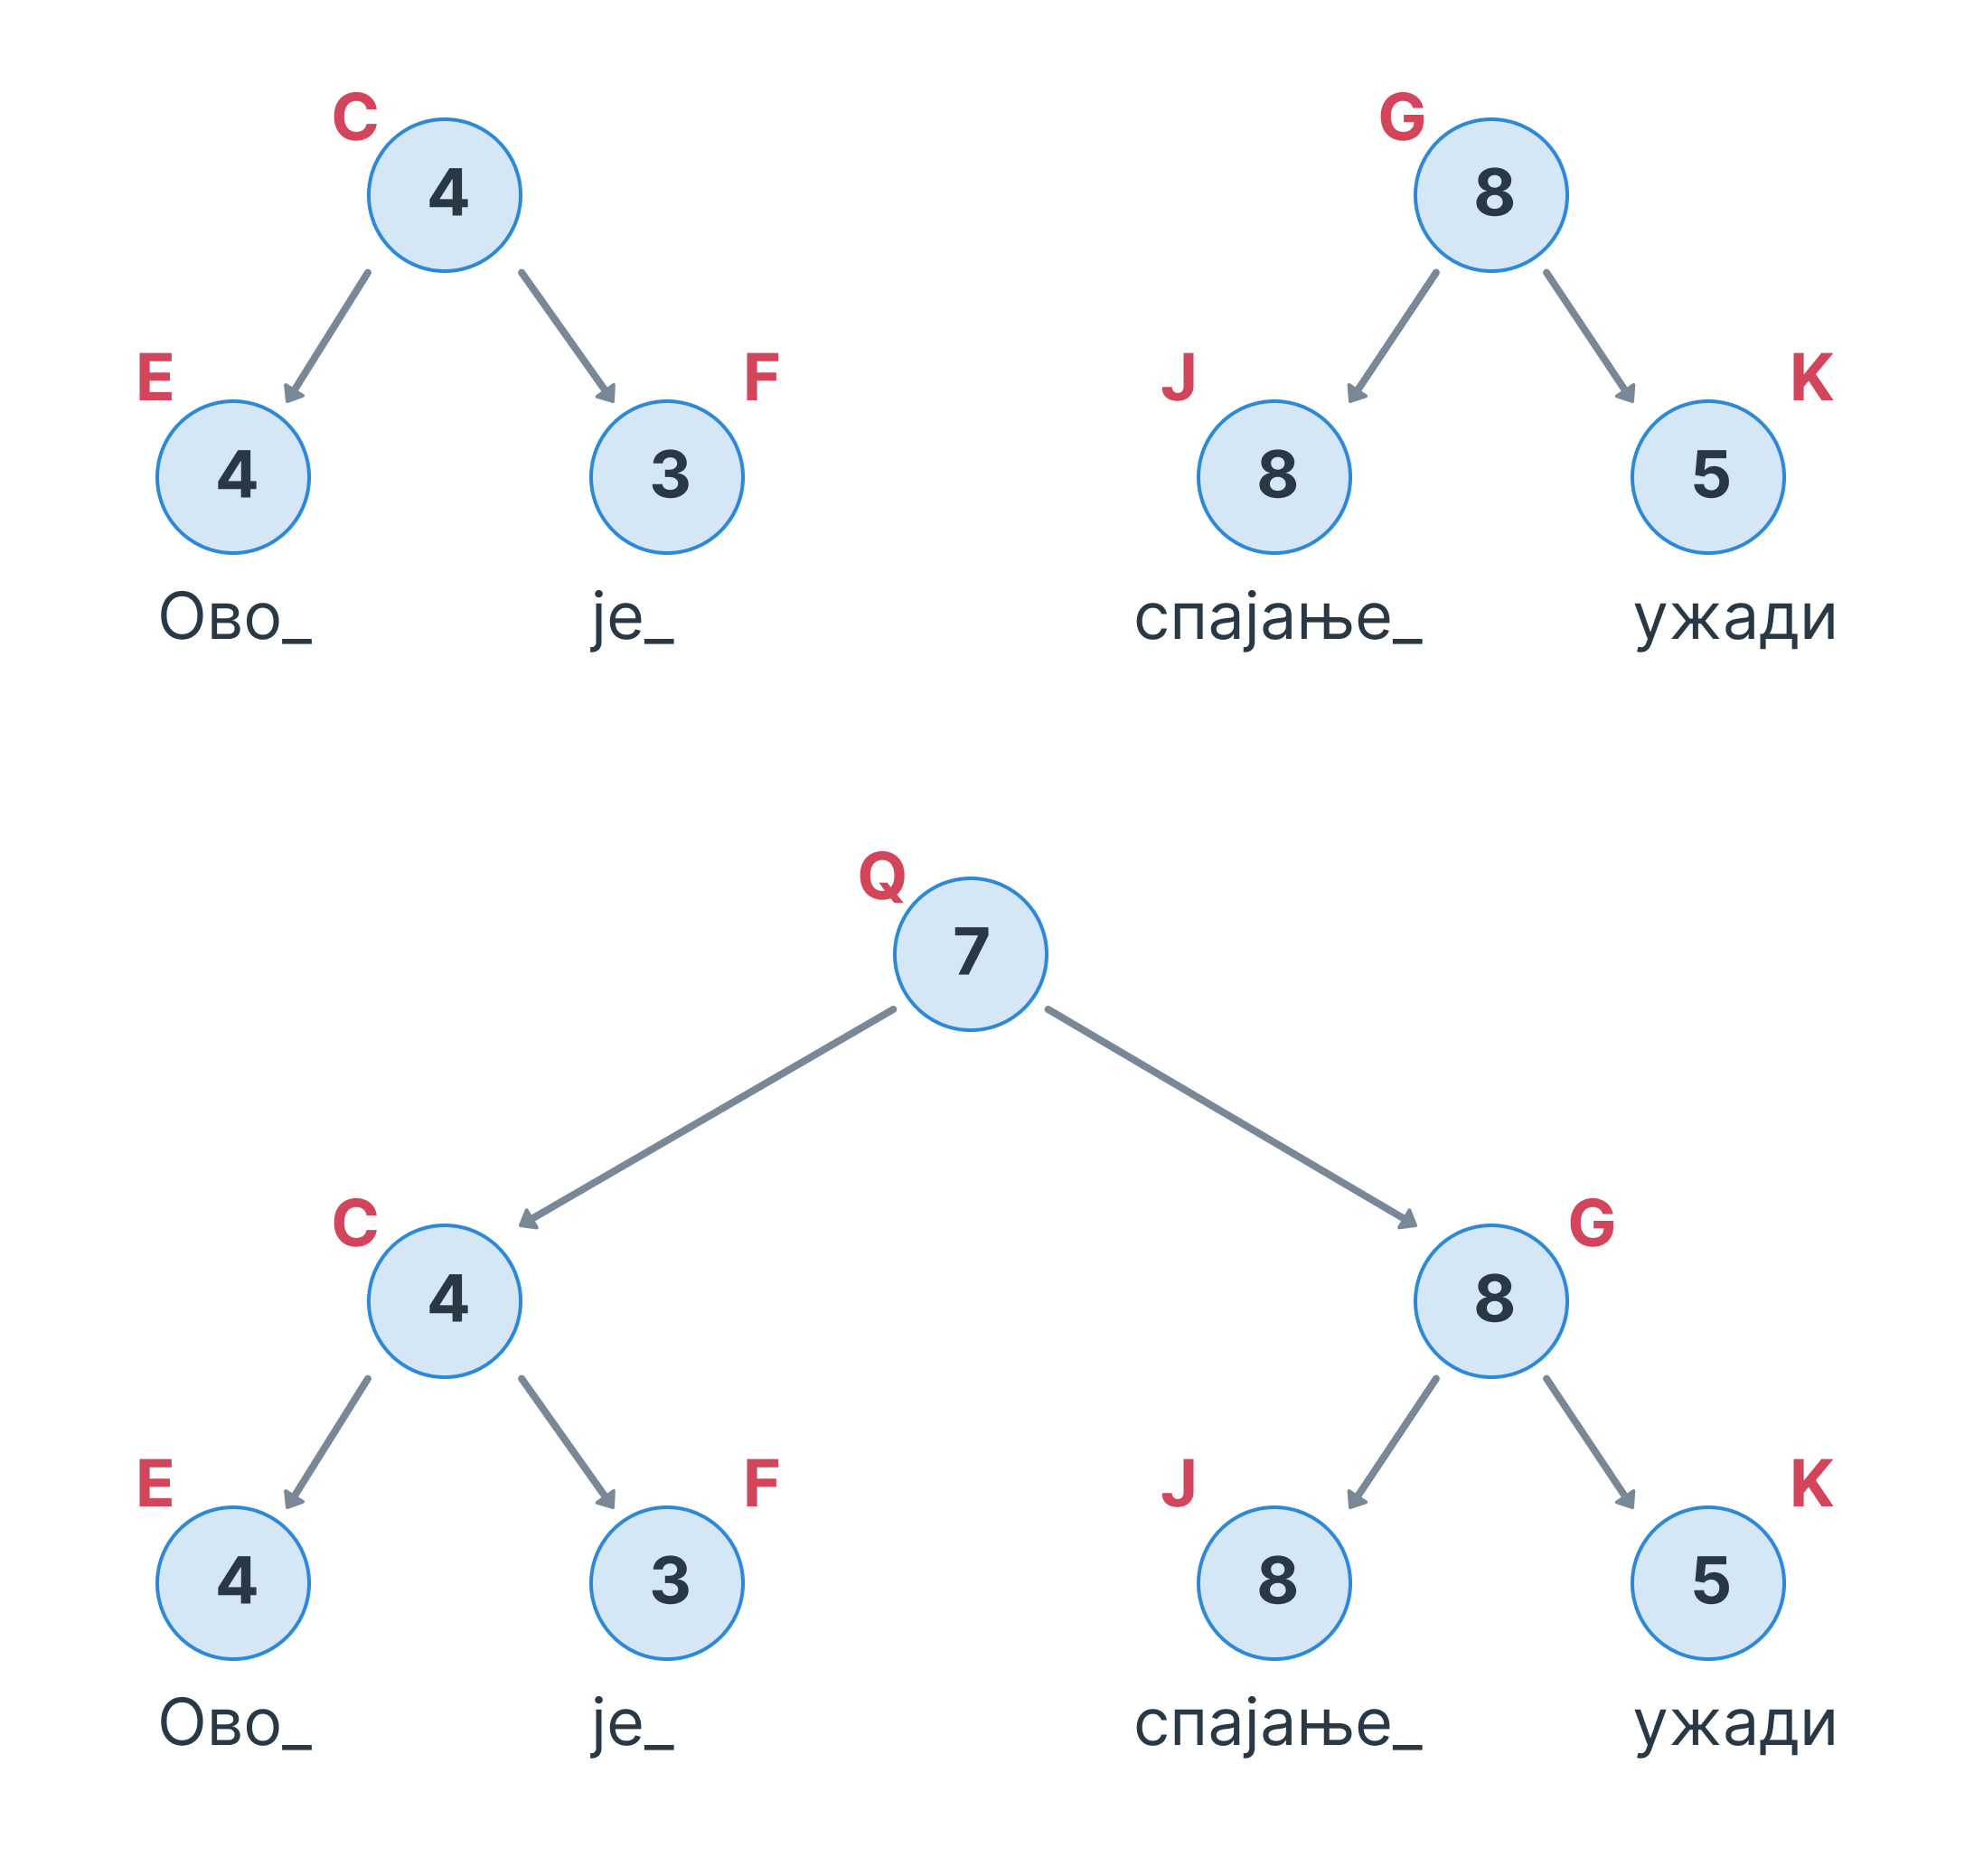
\includegraphics[width=0.7\textwidth]{images/rope_concat_1.png}
  \caption{Надовезивање два ужета}
  \label{fig:rope_concat}
\end{figure}

\subsection{Дељење}
\paragraph{}
\emph{Дељење} (енг. \begin{latinica}\textit{splitting}\end{latinica}) ужета \(r\) који
садржи текст \(t\) по
индексу \(i\) на два ужета, \(r_1\) и \(r_2\), који садрже текстове \(t_1\) и \(t_2\),
где \(t_1\) садржи карактере од почетка текста \(t\) до \(i\)-тог индекса (укључујући и
карактер на \(i\)-том индексу), а \(t_2\) садржи карактере десно од \(i\)-тог индекса па
до краја текста \(t\), врши се на следећи начин.

\paragraph{}
Најпре се налази \(i\)-ти карактер: ако је то последњи карактер ниске у листу онда се не ради ништа. У супротном се лист дели на два нова листа, где је \(i\)-ти карактер последњи
карактер ниске левог листа. Нека је лист чији је \(i\)-ти карактер последњи у нисци
означен са \(l_s\). Сада се листови деле у две групе \(L_1\) и \(L_2\). У \(L_1\) се налазе
листови лево од \(l_s\) као и сам \(l_s\), док се у \(L_2\) налазе листови десно од \(l_s\). Листови из групе \(L_2\) се одвајају од главног ужета и затим се спајају заједно.
Алгоритам се завршава тако што се балансирају два новодобијена ужета. Сложеност је иста као
код претходних операција. 


\begin{exmp}
На слици \ref{fig:ropе_split} је 
илустрован поступак дељења по индексу 10. Прво се проналази карактер на датом индексу на
начин описан у делу о претрази. Затим се проверава да ли је тај карактер последњи у листу,
па пошто јесте, врши се подела на \(l_1\) и \(l_2\) по том листу.

\begin{figure}
  \centering
  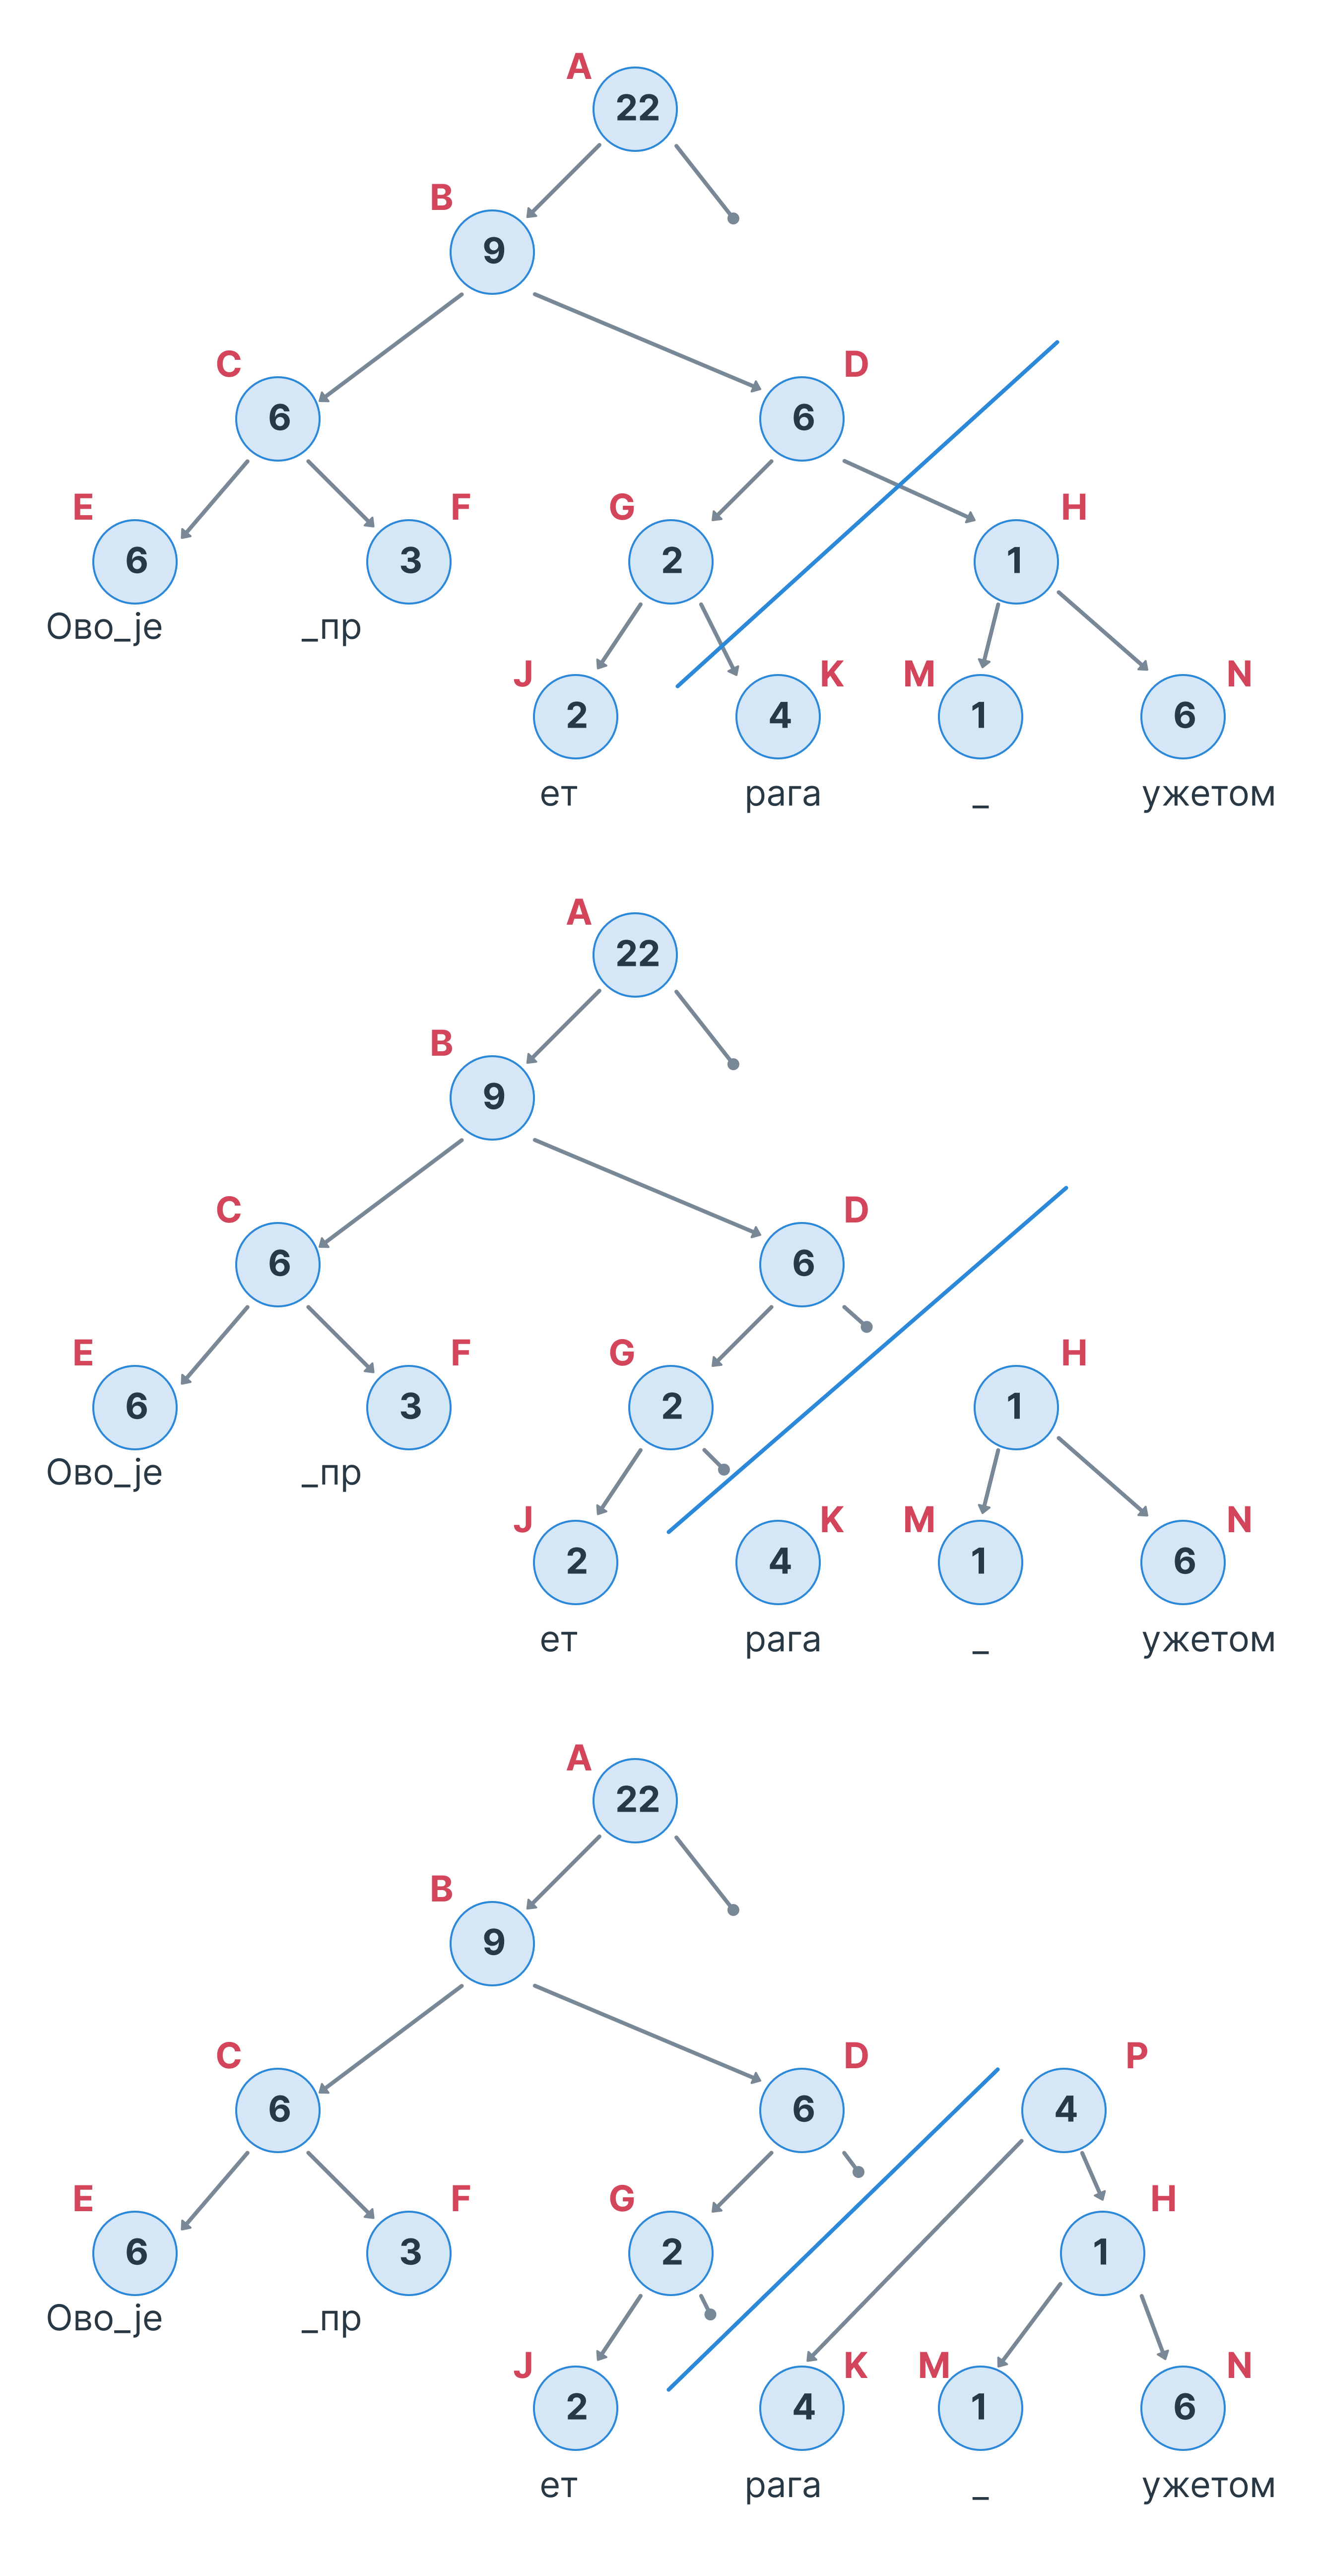
\includegraphics[width=0.8\textwidth]{images/rope_split_1.png}
  \caption{Дељење ужета по индексу 10}
  \label{fig:ropе_split}
\end{figure} 
\end{exmp}

\subsection{Уметање}
\paragraph{}
Да би се неки текст \(t\) уметнуо y уже \(r\) на индексу \(i\), довољно је да се искористе претходно дефинисане операције дељења и конкатенације. Најпре се уже \(r\)
подели по индексу \(i\), чиме се добијају два ужета \(r_1\) и \(r_2\), затим се на \(r_1\)
надовеже текст \(t\) и добија се ново уже \(r_3\). На крају се на уже \(r_3\) надовеже \(r_2\). Ова операција се састоји од три операције сложености \(O(\log{}n)\), тако да је
њена укупна сложеност \(O(\log{}n)\).

\subsection{Брисање}
\paragraph{}
Уколико је потребно обрисати сегмент текста \(t\) смештене ужету \(r\) који почиње на \(i\)-том карактеру, а завршава се на \((i+l)\)-том карактеру, онда се то може урадити у три корака. Прво се изврши дељење ужета \(r\) по индексу \(i\) на два ужета \(r_1\) и
\(r_2\), затим се \(r_2\) подели по \(l\)-том индексу на \(r_3\) и \(r_4\). 
У последњем кораку, надовезивањем \(r_1\) и \(r_4\) се добија коначан резултат. 
Из истих разлога као код уметања, сложеност операције је \(O(\log{}n)\).

\section{Табела делова}
\paragraph{}
\emph{Табела делова} (енг. \begin{latinica}\textit{piece table}\end{latinica}) је структура података која се састоји од два бафера у којима се налази текст и повезане 
листе чворова који показују на текст у баферу. Текст едитор који је имплементиран током
рада на овој тези користи ову структуру података, тако да ће она бити нешто детаљније
описана него претходне две структуре података.

\paragraph{}
У први бафер се учитава текст који се већ налазио у датотеци коју смо отворили и тај 
бафер се назива \emph{оригинални бафер} 
(енг. \begin{latinica}\textit{original buffer}\end{latinica}). 
Од тренутка учитавања текста из датотеке па надаље он остаје непромењен. 

\paragraph{}
У други бафер, који се назива \emph{бафер за додавање} 
(енг. \begin{latinica}\textit{add buffer}\end{latinica}), 
се додаје текст који се током времена уписује у текст едитор. Сваки пут
када се додаје текст, без обзира на то на ком месту теба извшити додавање, 
текст се додаје на крај бафера. Важно је напоменути да када се брише текст, он се не 
брише из бафера за додавање, већ остаје у њему. На овај начин се ни у ком моменту не 
јавља потреба да се врши померање текста који се већ налази унутар бафера.

\paragraph{}
Поставља се питање како је онда могуће исписати текст у правилном редоследу. То се постиже
коришћењем двоструко повезане листе чији су елементи тзв. \emph{дескриптори делова} (енг. \begin{latinica}\textit{piece descriptors}\end{latinica}). Сваки дескриптор садржи
информацију о томе на који од два бафера показује, на којем индексу бафера почиње текст и
колика је дужина тог текста. Следећи код приказује чланске променљиве класе \begin{latinica}\verb|PieceDescriptor|\end{latinica} у имплементацији рада.

\begin{minted}{c++}
class PieceDescriptor {
// ...
private:
    SourceType m_source;
    size_t m_start;
    size_t m_length;
};
\end{minted}

\paragraph{}
Предност ове структуре је што је једноставним операцијама, уметањем и брисањем чворова из
повезане листе, могуће ефикасно вршити измене текста. Мана је потенцијално велико меморијско заузеће бафера за додавање као и фрагментација на доста веома малих "делова",
што чини претрагу кроз листу мање ефикасном.

\paragraph{}
У наставку текста ће бити описане основне операције над овом структуром података. Најпре
ће бити уведене неке ознаке које ће бити употребљаване за све наведене операције:

\begin{itemize}
	\item \(n\) - дужина укупног текста,
	\item \(m\) - број елемената повезане листе,
	\item \(I_n \in \{0, 1,...,n-1\}\) - скуп валидних индекса текста,
	\item \(I_m \in \{0, 1,...,m-1\}\) - скуп валидних индекса повезане листе,
	\item \(p_i\) - почетак \(i\)-тог дескриптора, где је \(i \in I_m\),
	\item \(d_i\) - дужина \(i\)-тог дескриптора, где је \(i \in I_m\).
\end{itemize}

\subsection{Уношење текста}
\paragraph{}
Нека је потребно додати неки текст дужине \(d\) у текући текст почев од позиције
\(i \in \{0,1,...,n\}\), размотримо најпре два специјалана случаја за индекс \(i\):

\begin{enumerate}
	\item \(i=0\): У овом случају се додаје нови дескриптор на почетак листе.
	\item \(i=n\): У овом случају се додаје нови дескриптор на крај листе.
\end{enumerate}

За све остале случајеве пролази се кроз листу дескриптора слева на десно. 
Нека је сума дужина свих дескриптора пре \(ј\)-тог, при чему је \(j \in I_m\), једнака \(s_j\). Заустављамо се када буде важио услов \(s_j + d_j \geq i\), где је \(j\) индекс
елемента листе на ком се налазимо. Разликујемо два случаја:

\begin{enumerate}
	\item \(s_j + d_j = i\): У овом случају убацује се нови дескриптор испред \(j\)-тог
	елемента повезане листе дескриптора.
	\item \(s_j + d_j > i\): У овом случају се тренутни дескриптор дели на два тако
	да леви садржи \(i - s_j\) почетних карактера оригиналног дескриптора, а десни остале.
	Ово се постиже тако што се дужина \(j\)-тог дескриптора поставља на \(i - s_j\), затим
	се прави нови дескриптор чији је почетак \(p_j + (i - s_j)\), а дужина \(d_j - (i - s_j)\)
	и умеће се испред \(j\)-тог. На крају се додаје дескриптор са новим текстом између ова
	два.
	
\end{enumerate}

\paragraph{}
Сложеност ове операције је \(O(m + d)\), јер се кроз листу пролази највише \(m\) пута.
Додавање новог дескриптора и дељење претходног на два су операције сложености \(O(1)\), док
додавање новог текста дужине \(d\) у бафер има сложеност \(O(d)\).

\subsection{Брисање}
\paragraph{}
Брисање дела текста чији се индекси налазе у целобројном интервалу \([p, k)\), где су 
\(p \in I_n\), \(k \in I_n \cup \{n\}\), се врши аналогно уметању текста. 
Пролази се кроз повезану листу све док не буде испуњен услов \(s_i + d_i \geq p\) за неко 
\(i \in I_m\). Затим се редом пролази кроз све дескрипторе који садрже текст чији су индекси из опсега \([p_j, p_j+d_j)\) за \(ј \geq i\), \(j \in I_m\) и имају пресек са
\([p, k)\) и врши се њихово ажурирање на основу следећих правила:

\begin{enumerate}
	\item Ако је пресек суфикс опсега \([p_j, p_j+d_j)\) дужине \(d_p\), онда се одузима суфикс 
	од дескриптора тако што му се смањује дужина за \(d_p\).
	
	\item Ako je пресек префикс опсега \([p_j, p_j+d_j)\) дужине \(d_p\), онда се одузима префикс
	 од дескриптора тако што му се помера почетак у десно за \(d_p\) и смањује дужина за исто
	 толико.
	 
	\item Ако је пресек цео опсег \([p_j, p_j+d_j)\), онда се брише цео дескриптор.
	 
	\item Ако је \([p, k)\) садржан у \([p_j, p_j+d_j)\) и није ни префикс ни суфикс опсега,
	онда се дескриптор дели на два нова, где први садржи опсег \([p_j, p)\), а други 
	\([k, p_j+d_j)\).
\end{enumerate}
\paragraph{}
Пошто се брисањем мења један или више дескриптора у повезаној листи, треба
приметити нека правила везана за горе наведене случајеве. Ако се мења више дескиптора
у једном брисању, онда се они морају налазити на узастопним позицијама у повезаној листи.
Случај 1. може важити само за последњи дескриптор који ће бити промењен у брисању.
Аналогно, случај 2. може важити само за први који ће бити промењен, док случај 3. 
може важити за све које ће се променити. Уколико за неки дескриптор важи случај 4, 
онда је он једини дескриптор који ће се ажурирати.

\paragraph{}
Временска сложеност брисања текста је \(O(m)\), јер се пролази кроз највише \(m\)
елемената повезане листе и свако ажурирање дескриптора је сложености \(O(1)\).

\subsection{Исписивање}
\paragraph{}
Уколико је потребно да се испише целокупан текст на стандардни излаз или у неку датотеку,
то је могуће постићи на следећи начин. Пролази се кроз листу дескриптора од почетка до краја
и за сваки дескриптор се исписује подниска одговарајућег бафера која почиње на индексу 
\(p_j\) и има дужину \(d_j\), где је \(j \in I_m\). На слици \ref{fig:piece_table} се може
видети како изгледа приказ једног текста помоћу табеле делова.

\begin{figure}[!ht]
	\centering
	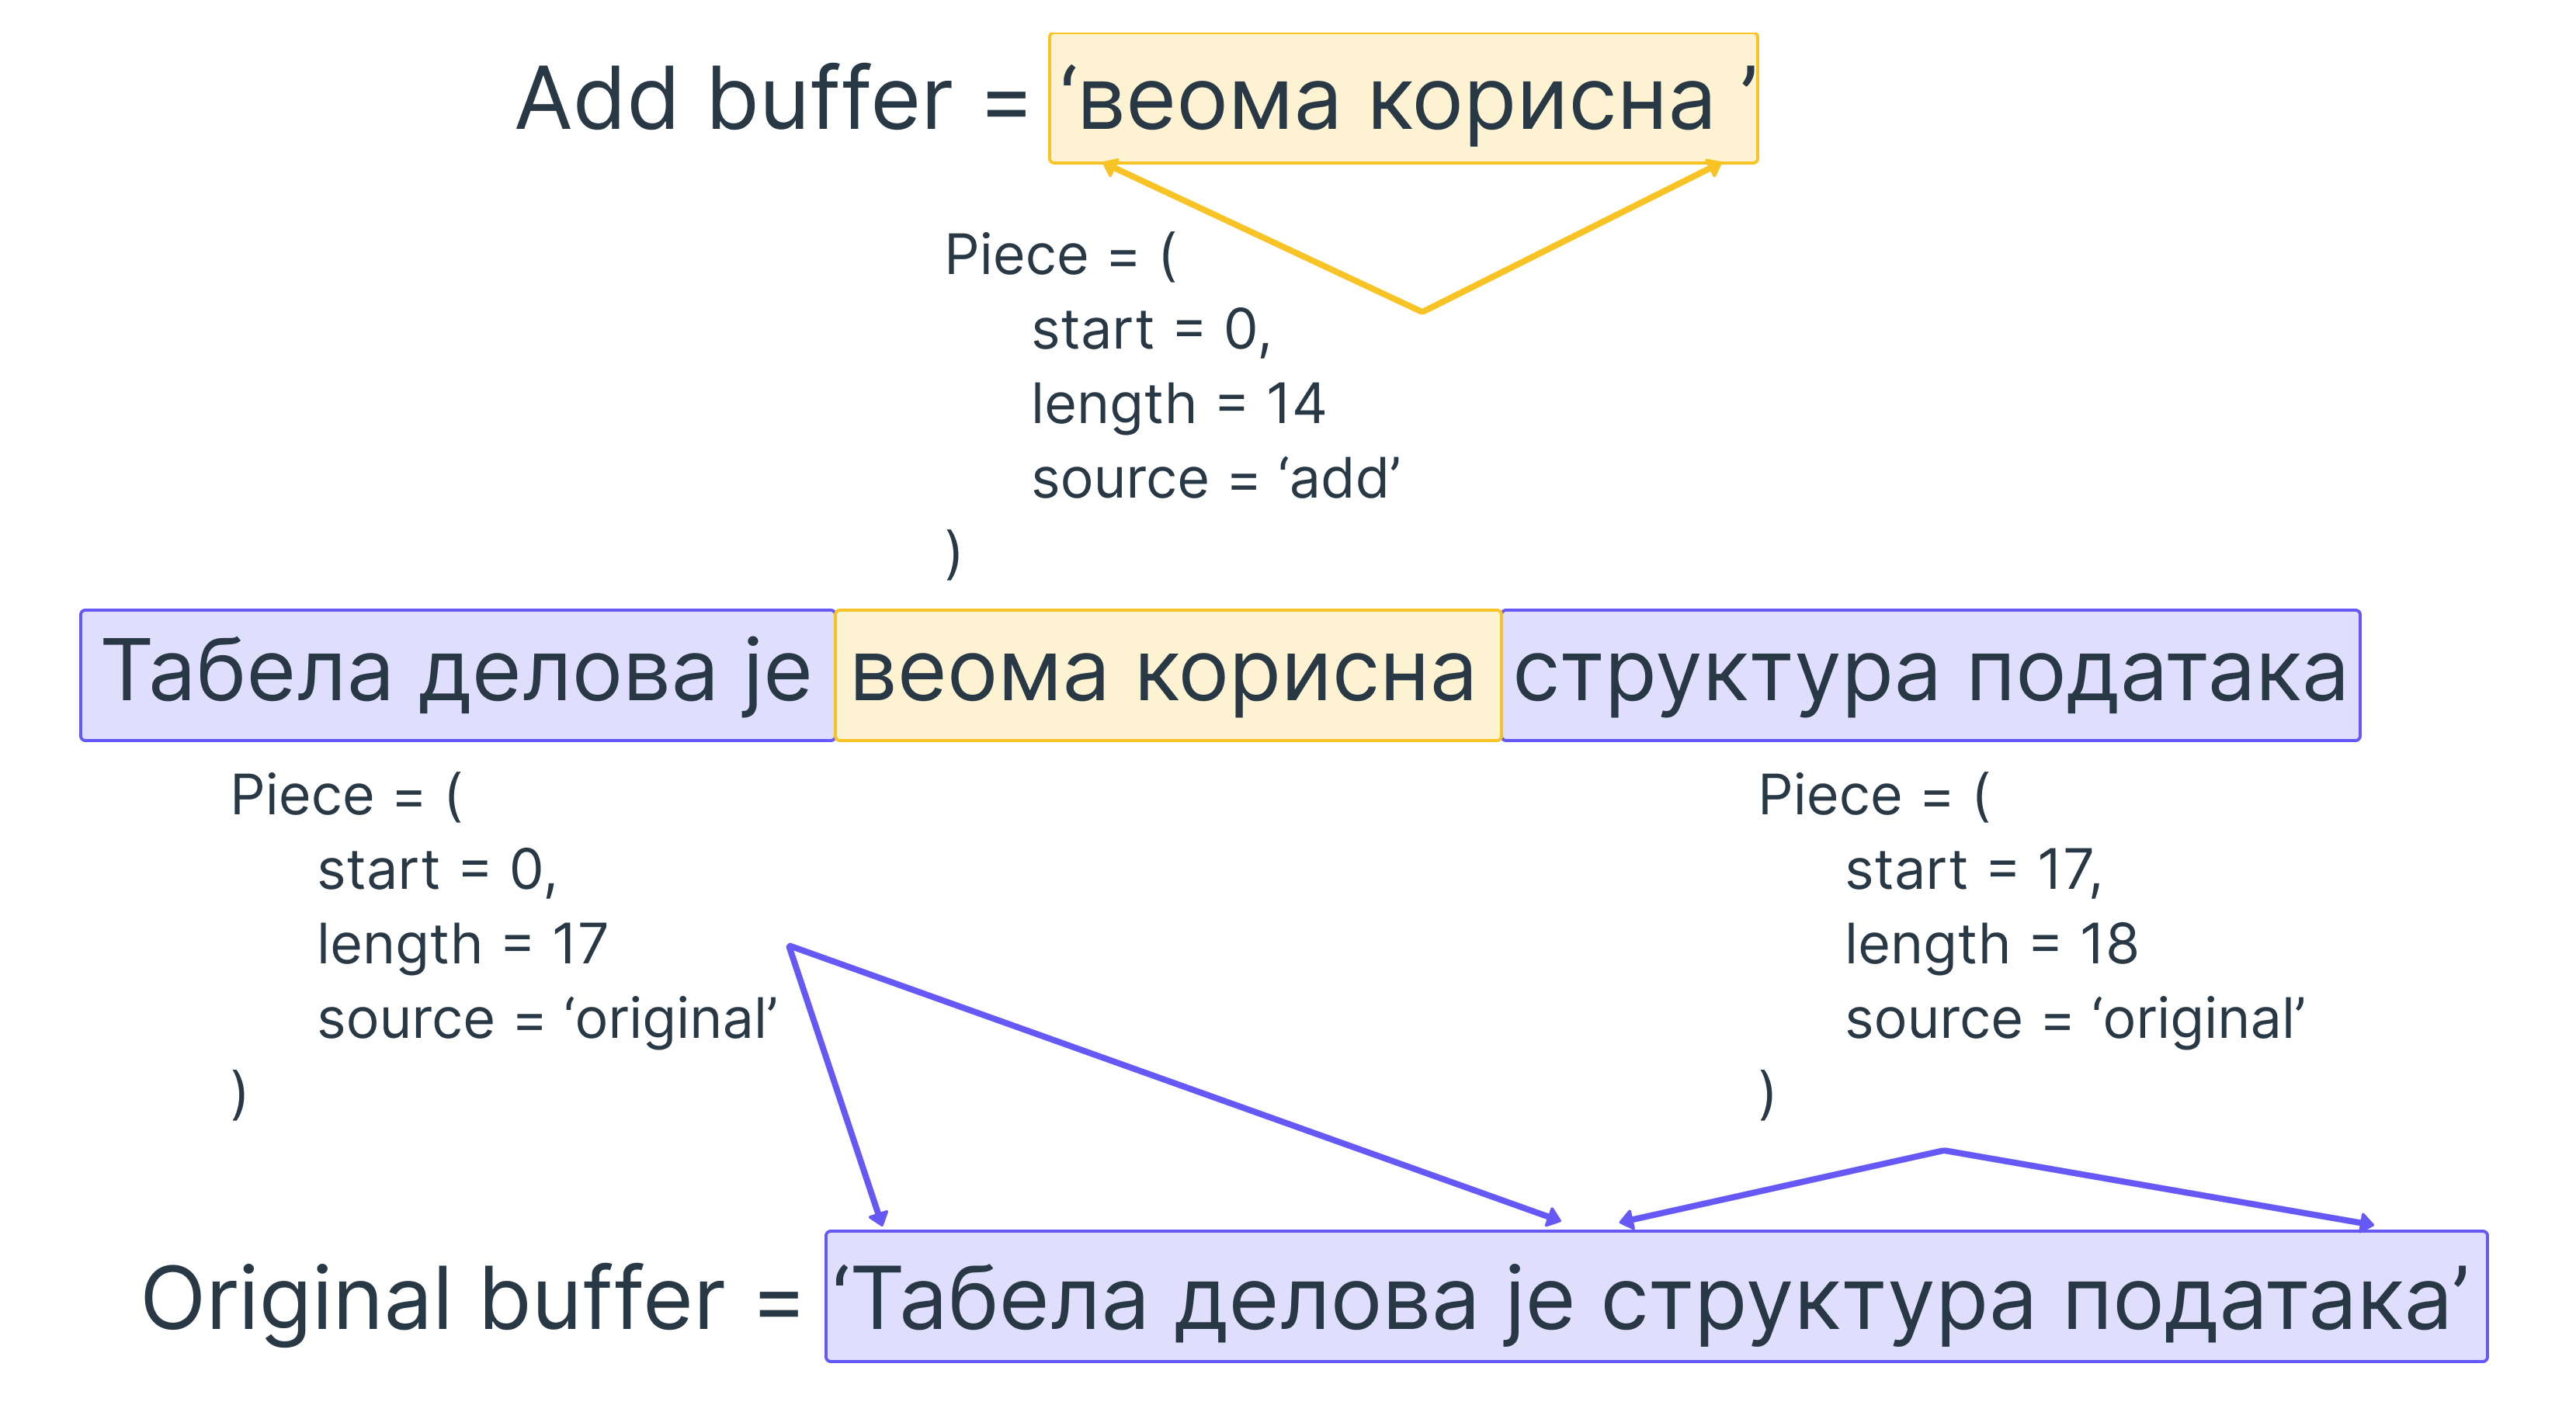
\includegraphics[width=1.0\textwidth]{images/piece_table_1.png}
	\caption{Приказ рада табеле делова}
	\label{fig:piece_table}
\end{figure}

\paragraph{}
По овом механизму по коме се целокупан текст добија надовезивањем "делова" бафера
је сама структура података добила име. Један од познатијих текст едитора који од 2018. 
користи табелу делова у својој имплементацији је \begin{latinica}\textit{Visual Studio Code}\end{latinica} \cite{VSC}.

\paragraph{}
Временска сложеност операције исписивања садржаја табеле делова је 
\(O(\sum_{i=0}^{m-1} d_i)\) тј. једнака је суми дужина свих дескриптора. 
Пошто је сума свих дужина једнака дужини укупног текста, онда се сложеност може
једноставније записати као \(O(n)\).

% ------------------------------------------------------------------------------
\chapter{Основне функционалности}
\label{chp:osnovne_funkcionalnosti}

\section{Обрада уноса}
\paragraph{}
Током уноса и обраде текста коришћењем едитора текста, корисник већину команди задаје преко тастатуре, док се мањи проценат њих задаје коришћењем миша. Један од задатака при 
имплементацији текст едитора јесте исправно обрадити све овакве уносе. 
Пре описа обраде, прво ће бити речи о самим карактерима и њиховим специфичностима. 

\subsection{Карактери}
\paragraph{}
За писање програмског кода најчешће се користи \begin{latinica}\textit{ASCII}\end{latinica} кодирање. \begin{latinica}\textit{ASCII}\end{latinica} табела представља стандард за кодирање
знакова који се користи за представљање текста у рачунарима. Она пресликава знакове
(слова, цифре, знакове интерпункције, контролне секвенце, итд.) у бројевне вредности,
омогућавајући на тај начин њихово чување и манипулацију у дигиталним системима. 
\begin{latinica}\textit{ASCII}\end{latinica} стандард користи 7 битова за представљање
сваког карактера, омогућавајући представљање 128 различитих карактера.


\paragraph{}
Немају сви карактери из \begin{latinica}\textit{ASCII}\end{latinica} табеле визуелну
репрезентацију: карактери чија је вредност у табели од 0 до 31 су тзв. \emph{контролни
карактери} (енг. \begin{latinica}\textit{control characters}\end{latinica}) који служе за
слање сигнала за комуникацију са периферним уређајима. Остали карактери, чија је вредност
између 32 и 127, се могу приказивати на излазу и њих називамо \emph{штампаним карактерима}
(енг. \begin{latinica}\textit{printable characters}\end{latinica}).
У табели \ref{tab:ascii} приказан је садржај \begin{latinica}\textit{ASCII}\end{latinica}
табеле.

\begin{table}[htbp]
\centering
\setlength{\extrarowheight}{8pt}
\begin{tabularx}{\linewidth}{|X| X | X | X | X | X | X | X | X | X | X | X | X | X | X | X | X|}
	\hline
	& \textbf{0} & \textbf{1} & \textbf{2} & \textbf{3} & \textbf{4} & \textbf{5} & \textbf{6} & \textbf{7} & \textbf{8} & \textbf{9} & \textbf{A} & \textbf{B} & \textbf{C} & \textbf{D} & \textbf{E} & \textbf{F} \\
	\hline
	\textbf{0x} & nul & soh & stx & etx & eot & enq & ack & bel & bs & ht & lf & vt & ff & cr & so & si \\
	\hline
	\textbf{1x} & dle & dc1 & dc2 & dc3 & dc4 & nak & syn & etb & can & em & sub & esc & fs & gs & rs & us \\
	\hline
	\textbf{2x} & sp & ! & \("\) & \(\#\) & \$ & \% & \& & ' & ( & ) & * & \(+\) & , & - & . & / \\
	\hline
	\textbf{3x} & 0 & 1 & 2 & 3 & 4 & 5 & 6 & 7 & 8 & 9 & : & ; & < & = & > & ? \\
	\hline
	\textbf{4x} & @ & A & B & C & D & E & F & G & H & I & J & K & L & M & N & O \\
	\hline
	\textbf{5x} & P & Q & R & S & T & U & V & W & X & Y & Z & [ & \texttt{$\backslash$} & ] & 
	\^{} & \_{} \\
	\hline
	\textbf{6x} & ` & a & b & c & d & e & f & g & h & i & j & k & l & m & n & o \\
	\hline
	\textbf{7x} & p & q & r & s & t & u & v & w & x & y & z & \{ & | & \} & \~{} & del \\
	\hline
\end{tabularx}
\caption{\begin{latinica}\textit{ASCII}\end{latinica} табела.}
\label{tab:ascii}
\end{table}

\subsection{Унос помоћу тастатуре}
\paragraph{}
Уколико корисник притисне неки тастер на тастатури, текст едитор ће га исписати само
ако тастер одговара штампаном карактеру или карактеру за форматирање текста (као што
су \begin{latinica}\textit{Tab}\end{latinica} и \begin{latinica}\textit{Enter}\end{latinica}). Сви остали тастери се игноришу
што омогућава да се неким од њих кодирају друге команде у едитору. 
Поред тога, могуће је комбиновање контролног и штампаног карактера како
би се кодирале додатне команде. Ово се постиже притиском на два или три тастера истовремено. Најчешће се врши комбиновање два тастера, где је први обично \begin{latinica}\textit{Ctrl}\end{latinica}.

\paragraph{}
У едитору текста имплеметираног при раду на тези, обраду ових уноса врши корисничка метода \begin{latinica}\verb|handleKeyboardInput()|\end{latinica} класе
\begin{latinica}\verb|TextEditor|\end{latinica}. Она врши периодичну проверу да ли
је притиснут један или више тастера у датом тренутку и да ли је том комбинацијом тастера 
задата нека специјална команда. Уколико јесте, извршава се одговарајућа команда. Ако
то није случај, утврђује се да ли је притиснут неки штампани карактер и уколико јесте,
прослеђује се методи за унос.


\subsection{Унос помоћу миша}
\paragraph{} 
Некада се команде задају и путем миша, најчешће ради померања \emph{курсора} 
(енг. \begin{latinica}\textit{cursor}\end{latinica}) и \emph{означавања текста}
(енг. \begin{latinica}\textit{text selection}\end{latinica}). Помоћу миша се такође 
може приступити менију у коме се налазе додатне команде и алати.
О курсору и означавању, као и додатним командама биће више речи у наставку рада.
Сигнали који се обрађују су тастер миша који је притиснут (леви, десни или средњи),
позиција курсора миша као и то да ли корисник користи један клик, дупли клик или
држи тастер миша.

\paragraph{}
Имлементација обраде уноса миша је сложенија него код обраде уноса са тастатуре. Метода
\begin{latinica}\verb|handleMouseInput()|\end{latinica}
класе \begin{latinica}\verb|TextEditor|\end{latinica} обрађује све догађаје
миша. Она се периодично позива и врши проверу да ли је корисник притиснуо леви тастер на 
мишу, уколико јесте активира се одговарајућа команда и прослеђује се позиција миша. 
Такође се проверава да ли је корисник држао леви тастер и уколико јесте, активира
одговарајућу методу и шаље две позиције миша, у тренутку када је дугме притиснуто и 
када је отпуштено. Joш једна врста обраде уноса миша је померање \emph{точкића} (енг. \begin{latinica}\textit{mouse wheel}\end{latinica}) којим се врши хоризонтално и 
вертикално скроловање (енг. \begin{latinica}\textit{scrolling}\end{latinica}), док
десни тастер није употребљен у овој имплементацији.


\section{Курсор} \label{cursor}
\paragraph{}
Један од основних елемената сваког едитора текста јесте курсор. Његова функција је да
означи место у тексту на којем ће бити извршена следећа измена. Углавном је представљен у 
виду уређеног пара реда и колоне у којој се курсор налази. Иако су у овом раду до сада
измене представљане помоћу индекса неког низа карактера, репрезентација у виду уређеног
пара је интуитивнија и прегледнија за корисника. Стога се ова репрезентација користи и
у класи \begin{latinica}\verb|TextCoordinates|\end{latinica} едитора текста имплементираног
при раду на тези.

\begin{minted}{c++}
class TextCoordinates {
	// ...
	public:
	size_t m_row;
	size_t m_col;
};
\end{minted}

\paragraph{}
Треба, такође, напоменути да у овој репрезентацији обе кординате починњу од
један, а не од нула као код индекса, као и да се вредност колоне може кретати
у целобројном интервалу \([1, d+1]\), где је \(d\) дужина тренутног реда на ком се
курсор налази.

\paragraph{}
Курсор се на већини данашњих рачунара помера позиционирањем миша на жељено место
и притиском на леви тастер или, алтернативно, помоћу стрелица на тастатури. Такође, 
притиском на тастере \begin{latinica}\textit{Home}\end{latinica} и
\begin{latinica}\textit{End}\end{latinica} врши се померање курсора на почетак, односно на крај тренутног реда. У наредном програмском коду илустроване су неке од метода за померање
курсора, док се на слици \ref{fig:cursor} може видети курсор у текст едитору представљен
белом усправном цртом. У статусној линији (на доњем делу едитора) могу се видети тренутне координате курсора, тј. редни број његове врсте и колоне.

\begin{minted}{c++}
class Cursor {
public:
	//...
	void moveRight(size_t times = 1);
	void moveLeft(size_t times = 1);
	void moveUp(size_t times = 1);
	void moveDown(size_t times = 1);
	void moveToBeginning();
	void moveToEnd();
	void moveToEndOfFile();
	//...
};
\end{minted}

\begin{figure}[!ht]
	\centering
	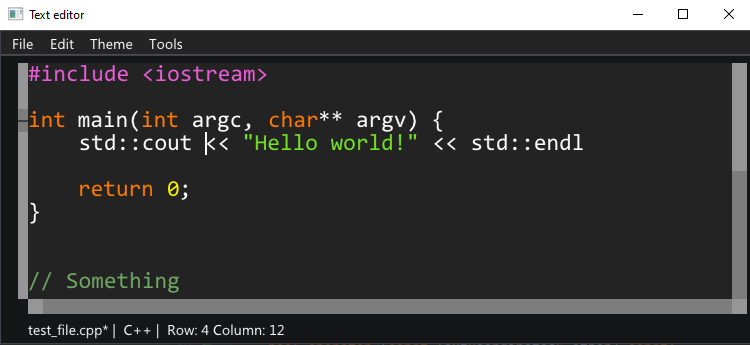
\includegraphics[width=1.0\textwidth]{images/cursor.png}
	\caption{Приказ курсора у текст едитору}
	\label{fig:cursor}
\end{figure}

\section{Операције са појединачним карактерима}

\subsection{Унос}
\paragraph{}
Једна од основних функционалности текст едитора је уношење текста карактер
по карактер. Тај унос се врши тако што корисник притиска тастер за одговарајући
штампани карактер и он се уноси на тренутну позицију курсора, тј. испред карактера на ком се налази курсор, уколико није на крају реда, када се уноси иза последњег карактера. 

\paragraph{}
Унос се имплементира тако што се дохвате координате курсора и проследе функцији
\begin{latinica}\verb|textCoordinatesToBufferIndex(TextCoordinates coords)|\end{latinica} 
која преводи уређени пар врсте и колоне у индекс континуалног низа карактера. То се постиже на
следећи начин: вредност индекса се иницијализује на 0, а затим се пролази кроз све редове
изнад тренутног, почевши од првог, и на индекс се додаје \(d+1\) (додаје се један да би се урачунао и знак за нови ред), где је \(d\) дужина тог реда. 
Када се стигне до тренутног реда вредност индекса се увећава за вредност колоне умањене за
један. Наредни програмски код илуструје рад ове функције.

\begin{minted}{c++}
size_t LineBuffer::textCoordinatesToBufferIndex
(const TextCoordinates &coords) const {
		
	size_t index = 0;
	
	for (size_t i=0; i < coords.m_row-1; i++)
		index += lineAt(i).size() + 1;
	
	index += (coords.m_col - 1);
	
	return index;
}
\end{minted}

\paragraph{}
Када је добијен индекс низа карактера, он се прослеђује табели делова заједно са  притиснутим карактером и врши се унос и курсор се помера за једно место у десно. 
На примеру функције 
\begin{latinica}\verb|insertCharToPieceTable|\end{latinica} која припада класи
\begin{latinica}\verb|TextBox|\end{latinica} се може видети поступак уметања
карактера у табелу делова.

\begin{minted}{c++}
bool TextBox::insertCharToPieceTable(char c) {
	auto coords = m_cursor->getCoords();
	size_t index = m_lineBuffer->textCoordinatesToBufferIndex(coords);
	return m_pieceTableInstance->getInstance().insertChar(c, index);
}
\end{minted}


\subsection{Брисање}
\paragraph{}
Брисање поједначних карактера се врши тако што корисник позиционира курсор
на жељено место и притисне тастер за брисање карактера. Треба напоменути да 
постоје два тастера за брисање карактера, то су \begin{latinica}\textit{Backspace}\end{latinica}
и \begin{latinica}\textit{Delete}\end{latinica}.
\begin{latinica}\textit{Backspace}\end{latinica} брише карактер лево од курсора,
док \begin{latinica}\textit{Delete}\end{latinica} брише онај на позицији курсора.
После брисања се у првом случају курсор помера за једно место у лево, док у другом
случају остаје на истој позицији. Брисање је имплементирано на сличан начин као унос.

\paragraph{}
Текст едитор који је имплементиран током рада на овој тези користи две одвојене
методе за обе врсте брисања. То су 
\begin{latinica}\verb|backspace()| \end{latinica} и
\begin{latinica}\verb|deleteChar()| \end{latinica} класе
\begin{latinica}\verb|TextBox| \end{latinica}.

\begin{minted}{c++}
void TextBox::backspace() {
	auto deleted = deleteSelection();
	
	if (deleted)
		return;
	
	auto coords = m_cursor->getCoords();
	size_t index = m_lineBuffer->textCoordinatesToBufferIndex(coords);
	
	if (index != 0) {
		updateUndoRedo();
		m_pieceTableInstance->getInstance().flushInsertBuffer();
		
		auto initialized = 
			m_pieceTableInstance->getInstance().backspace(index);
		
		if (initialized)
		m_cursor->recordCursorPosition();
		
		updateStateForTextChange(false, 1, m_cursor->getRow());
		m_cursor->moveLeft();
		updateStateForCursorMovement();
	}
}
\end{minted}

\section{Означавање текста}
\paragraph{}
Означавање текста је функционалност која кориснику пружа могућност означавања
неког непрекидног сегмента текста ради брисања или \emph{копирања}
(енг. \begin{latinica}\textit{copy}\end{latinica}). Копирање ће бити
објашњено у наставку рада. Означавање текста се најчешће врши помоћу миша, тако што корисник превлачи курсор миша преко дела екрана у коме се налази текст који жели да изабере
и унесе команду за брисање или копирање. Означавање текста се може вршити и помоћу тастатуре,
тако што корисник држи тастер \begin{latinica}\textit{Shift}\end{latinica} и стрелицама
помера курсор. У овом случају се памти позиција курсора у тренутку када је притиснут тастер 
и она ће представљати један крај означеног текста. Други крај означеног текста ће бити позиција на коју је корисник померио курсор држећи тастер
\begin{latinica}\textit{Shift}\end{latinica}.

\paragraph{}
Пре него што буде објашњена импементација, прво ће бити дефинисан поредак између текстуалних координати, о којима је било речи у одељку \ref{cursor}. Пошто су координате
представљене уређеним паром реда и колоне,  оне се тако и пореде. Прво се пореде вредности редова, па уколико су оне једнаке, онда се пореде вредности колоне. У следећем коду
илустрована је дефиниција поређења за операторе \(=\) и \(<\). Симетрични оператори се дефинишу аналогно.

\begin{minted}{c++}
bool TextCoordinates::operator==(const TextCoordinates &other) const {
	return m_row == other.m_row && m_col == other.m_col;
}

bool TextCoordinates::operator<(const TextCoordinates &other) const {
	return (m_row < other.m_row) 
	|| (m_row == other.m_row && m_col < other.m_col);
}
\end{minted}

Oзначавање непрекидног дела текста је у едитору ЈЕТ представљено помоћу две текстуалне координате. Прва координата представља локацију на којој почиње текст који је
означен, а друга локацију где се завршава. Треба нагласити да почетак мора бити мањи или једнак од краја. Потребно је, такође, чувати информацију о томе да ли је означени текст активан. У следећем коду илустрован је пример чланских променљивих класе 
\begin{latinica}\verb|Selection|\end{latinica}.

\begin{minted}{c++}
class Selection {
//...
private:
	bool m_active;
	bool m_rectangular;
	TextPosition m_start;
	TextPosition m_end;
};
\end{minted}


\paragraph{}
Када метода \begin{latinica}\verb|handleMouseInput()|\end{latinica} детектује држање
левог тастера, она прослеђује две позиције миша методи \begin{latinica}\verb|setMouseSelection()|\end{latinica} класе
\begin{latinica}\verb|TextBox|\end{latinica}. Онда она на основу те две позиције
рачуна на које текстуалне координате оне показују и додељује мању од вредности координати
која означава почетак, а већу координати која означава крај. 
На крају се означени текст обележава као активан.

\paragraph{}
Уколико је означени текст активан и корисник кликне било где на текстуално поље едитора,
он се деактивира. Тренутно означени текст се може деактивирати и притиском на стрелице за померање курсора. При притиску на тастере за брисање док је означени текст активан, сав означени текст се брише. Исто важи и за операције \emph{исецања}
(енг. \begin{latinica}\textit{cut}\end{latinica}) и \emph{налепљивања}
(енг. \begin{latinica}\textit{paste}\end{latinica}). Деактивирање означеног текста
се имплементира тако што се чланска променљива 
\begin{latinica}\verb|m_active|\end{latinica} постави на вредност
\begin{latinica}\verb|false|\end{latinica}.

\paragraph{}
Притиском на комбинацију тастера \begin{latinica}\textit{Shift}\end{latinica} и
\begin{latinica}\textit{Home}\end{latinica} се почетак означавања поставља на почетак 
текућег реда, а крај на тренутну позицију курсора, док се притиском на тастере 
\begin{latinica}\textit{Shift}\end{latinica} и \begin{latinica}\textit{End}\end{latinica}
почетак означеног текста поставља на позицију курсора, а крај на последњу колону у текућем
реду. Притиском на комбинацију тастера \begin{latinica}\textit{Ctrl}\end{latinica} и
\begin{latinica}\textit{A}\end{latinica} означава се читав текст. На слици 
\ref{fig:selection} се може видети пример означавања, где је означени текст
уоквирен правоугаоником другачије боје од позадине.

\begin{figure}[!ht]
	\centering
	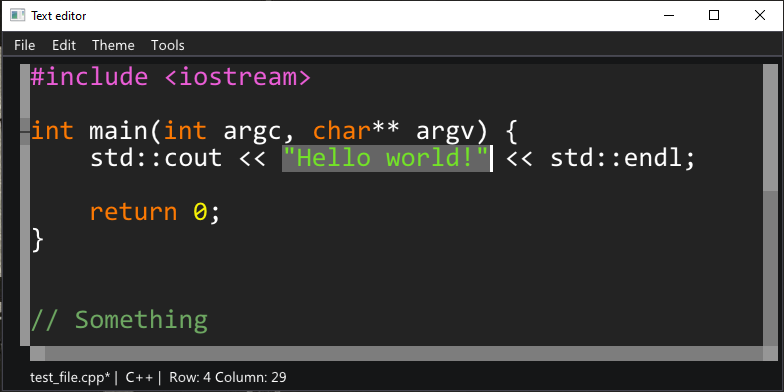
\includegraphics[width=1.0\textwidth]{images/selection.png}
	\caption{Приказ означавања у текст едитору}
	\label{fig:selection}
\end{figure}

\section{Управљање текстуалним датотекама}
\paragraph{}
Сврха едитора текста јесте мењање текстуалних датотека или креирање нових. 
Како би то било могуће, потребно је кориснику обезбедити могућност да креира нову или 
отвори постојећу датотеку. Потребно је и омогућити чување измена које корисник
прави као и могућност избора локације на којој ће датотека бити сачувана. У наредним 
одељцима биће обрађене те функционалности. Овим функционалностима се приступа путем
менија који се налази испод насловне линије, на слици \ref{fig:file_menu} илустрован је мени за управљање датотекама у оквиру едитора ЈЕТ.

\begin{figure}[!ht]
	\centering
	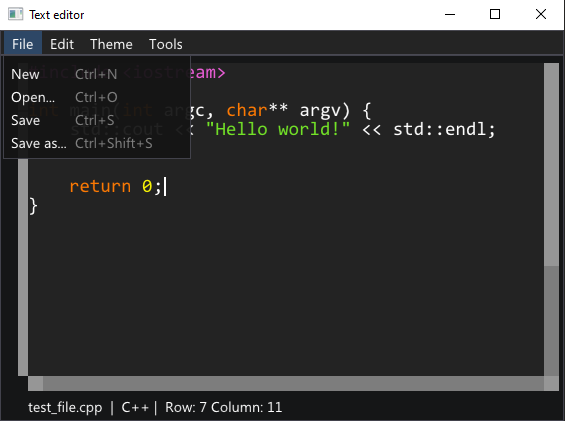
\includegraphics[width=1.0\textwidth]{images/file_menu.png}
	\caption{Приказ менија за управљање датотекама}
	\label{fig:file_menu}
\end{figure}

\subsection{Чување датотека}
\paragraph{}
Корисник може сачувати тренутни садржај едитора у датотеку притиском на дугме 
\begin{latinica}\textit{Save}\end{latinica} у менију или комбинацијом
тастера \begin{latinica}\textit{Ctrl}\end{latinica} и
\begin{latinica}\textit{S}\end{latinica}. Тренутни садржај се чува на 
жељеној локацији, а уколико иста није дефинисана, тражи се од корисника
да је унесе. Такође је дозвољено и чување тренутне датотеке на новој локацији
притиском на дугме \begin{latinica}\textit{Save as}\end{latinica} у менију, при
чему је поступак исти као и у случају када путања није унапред дефинисана.

\paragraph{}
Чување датотека у оквиру едитора ЈЕТ извршава метода
\begin{latinica}\verb|save()|\end{latinica} класе \begin{latinica}\verb|TextEditor|\end{latinica}. Она проверава да ли је дефинисана 
путања и уколико није, прослеђује извршавање функцији \begin{latinica}\verb|saveAs()|\end{latinica}. Ако је путања дефинисана, извршавање
се наставља у истоименој функцији класе  \begin{latinica}\verb|TextBox|\end{latinica}.
Имплементација ове две истоимене функције, као и функције \begin{latinica}\verb|saveToFile()|\end{latinica}, илустрована је у следећем програмском коду.

\begin{minted}{c++}
void TextEditor::save() {
	if (m_activeTextBox->getFile() == nullptr)
		saveAs();
	else {
		m_activeTextBox->save();
		m_inactiveTextBox->save();
	}
}

bool TextBox::save() {
	m_dirty = false;
	
	m_pieceTableInstance->getInstance().flushInsertBuffer();
	m_pieceTableInstance->getInstance().flushDeleteBuffer();
	
	return saveToFile();
}

bool TextBox::saveToFile() {
	std::stringstream strStream;
	strStream << m_pieceTableInstance->getInstance();
	std::string buffer = strStream.str();
	
	return File::writeToFile(buffer, m_file->getPath());
}
\end{minted}



\paragraph{}
Када путања није дефинисана позива се метода \begin{latinica}\verb|saveAs()|\end{latinica}.
Она отвара дијалог у коме корисник треба да изабере локацију на којој ће бити сачувана
датотека и враћа њену путању. Уколико није дефинисана, \emph{екстензија}
(енг. \begin{latinica}\textit{extension}\end{latinica}) датотеке биће
постављена на обичну текстуалну датотеку (\begin{latinica}\textit{.txt}\end{latinica}).
Затим се позива истоимена метода класе \begin{latinica}\verb|TextBox|\end{latinica} која
поставља нову путању и уписује садржај едитора на дату локацију. Имплементација обе
методе са именом \begin{latinica}\verb|saveAs()|\end{latinica} илустрована је у 
наредном примеру кода.

\begin{minted}{c++}
void TextEditor::saveAs() {
	auto path = saveFileDialog();
	
	if (!path.empty()) {
		if (path.find_last_of('.') == std::string::npos)
		path += ".txt";
		m_activeTextBox->saveAs(path);
		m_inactiveTextBox->saveAs(path);
	}
}

bool TextBox::saveAs(std::string &filePath) {
	auto oldFile = m_file;
	m_file = new File(filePath);
	m_lineBuffer->setLanguageMode(
		File::getModeForExtension(m_file->getExtension())
	);
	delete oldFile;
	
	return save();
}
\end{minted}

\paragraph{}
Како би се водила евиденција о изменама у тренутној датотеци користи
се индикатор који се назива \emph{прљави бит} (енг. \begin{latinica}\textit{dirty bit}\end{latinica}). Он се активира уколико постоје неке измене које нису сачуване.
Када корисник отвара датотеку, прљави бит је неактиван.
Сваком променом текста активира се прљави бит, док се сваким
чувањем деактивира. Он је обично представљен карактером звездице поред
имена тренутно отворене датотеке у статусној линији.

\subsection{Отварање нове датотеке}
\paragraph{}
Корисник може отворити нову датотеку притиском на дугме 
\begin{latinica}\textit{New file}\end{latinica} у менију или комбинацијом тастера
\begin{latinica}\textit{Ctrl}\end{latinica} и
\begin{latinica}\textit{N}\end{latinica}. Када корисник покрене ову акцију,
тренутна датотека се затвара и уколико је активан прљави бит, едитор отвара
дијалог у коме корисника пита да ли жели да сачува измене. Затим се садржај
текстуалног поља као и табеле делова ресетује и курсор се поставља на почетак.

\paragraph{}
Ова функционалност је имплементирана у оквиру едитора ЈЕТ путем методе
\begin{latinica}\verb|newFile()|\end{latinica} класе
\begin{latinica}\verb|TextEditor|\end{latinica}. Она проверава да ли је фајл
сачуван и позива методу
\begin{latinica}\verb|handleFileNotSaved()|\end{latinica} 
уколико није. Затим позива истоимену методу класе \begin{latinica}\verb|TextBox|\end{latinica} која ресетује свој садржај.
У наредном примеру кода приказане су обе описане методе.

\begin{minted}{c++}
void TextEditor::newFile() {
	auto id = handleFileNotSaved();
	if (id == IDCANCEL)
		return;
	
	m_activeTextBox->newFile();
	if (m_splitScreen)
		m_inactiveTextBox->setFile(m_activeTextBox->getFile());
}

void TextBox::newFile() {
	m_pieceTableInstance->newFile();
	
	m_lineBuffer->getLines();
	m_cursor->clearUndoAndRedoStacks();
	m_cursor->setCoords({1, 1});
	m_scroll->updateScroll(m_width, m_height);
	m_scroll->updateMaxScroll(m_width, m_height);
}
\end{minted}

\subsection{Отварање постојеће датотеке}
\paragraph{}
Уколико корисник жели да отвори постојећу датотеку он може то учинити притиском
на дугме \begin{latinica}\textit{Open}\end{latinica} у менију или комбинацијом
тастера \begin{latinica}\textit{Ctrl}\end{latinica} и \begin{latinica}\textit{O}\end{latinica}. Када покрене ову команду, кориснику
се приказује дијалог у коме може изабрати датотеку коју жели и она се отвара у едитору текста . На слици \ref{fig:file_dialog} илустрован је дијалог за избор датотеке у едитору текста. Ову функционалност имплементира метода \begin{latinica}\verb|open()|\end{latinica} класе \begin{latinica}\verb|TextEditor|\end{latinica} и илустрована је наредним фрагментом кода.

\begin{figure}[!ht]
	\centering
	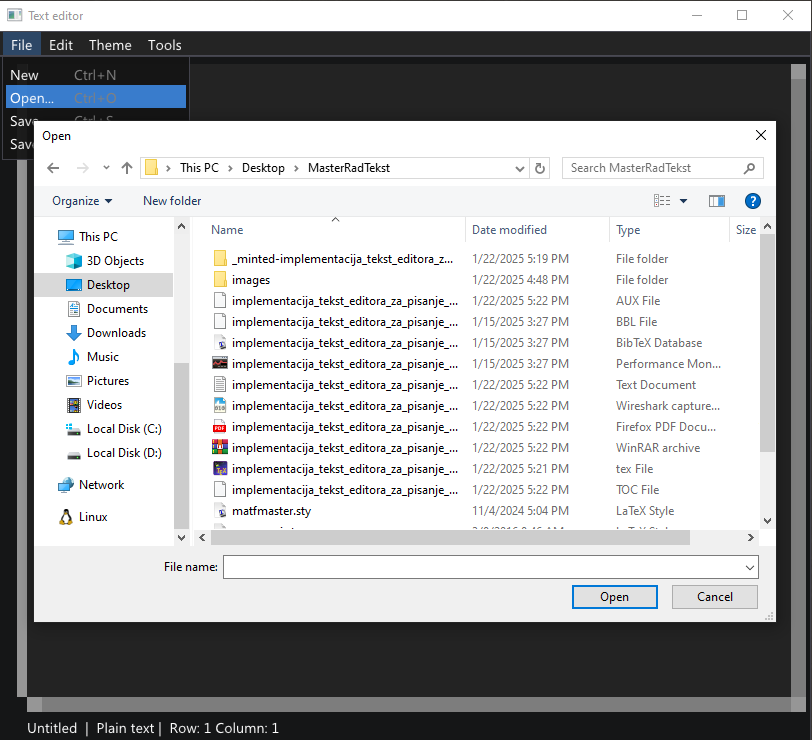
\includegraphics[width=1.0\textwidth]{images/file_dialog.png}
	\caption{Приказ дијалога за избор датотеке}
	\label{fig:file_dialog}
\end{figure}

\begin{minted}{c++}
void TextEditor::open() {
	auto id = handleFileNotSaved();
	if (id == IDCANCEL)
		return;
	
	auto path = openFileDialog();
	
	if (!path.empty()) {
		m_activeTextBox->open(path);
		m_inactiveTextBox->open(path);
	}
}
\end{minted}

\paragraph{}
Прво се проверава прљави бит, и уколико је активан отвара дијалог за чување помоћу
функције \begin{latinica}\verb|handleFileNotSaved()|\end{latinica}. Затим се 
отвара дијалог за избор датотеке помоћу функције
\begin{latinica}\verb|openFileDialog()|\end{latinica}  и враћа се изабрана
путања. На крају се позива истоимена метода класе
\begin{latinica}\verb|TextBox|\end{latinica} којом се отвара датотека и њен садржај
учитава у едитор.

\section{Исецање, копирање и налепљивање}
\paragraph{}
Исецање, копирање и налепљивање су операције које раде са привременом меморијом, 
која је део меморије у оперативним системима који је резервисан за привремено чување 
као и пренос података унутар једног или између више програма. Ти подаци могу бити текст,
слике, датотеке, итд. У овом одељку ћемо се бавити преносом текста. Привремена 
меморија функционише тако што по потреби можемо писати у њу или читати из ње. 
Обично се у једном тренутку може налазити само један податак у привременој меморији.

\paragraph{}
Када су ове три операције уведене у едиторе текста током седамдесетих година 
прошлог века, представљале су велико унапређење у ефикасности писања кода.
Корисници су сада могли да ефикасно померају делове текста по потреби као
и да копирају неке сличне фрагменте кода који се често користе уместо да их
пишу изнова, штедећи доста времена програмерима. У данашње време се едитори текста не
могу замислити без ових функционалности, што говори о њиховој корисности и широкој
употреби.
%Ове три операције представљају једне од највећих предности коришћења текст едитора,
%јер омогућавају копирање великих делова текста и њихово премештање. Код писања %к\^{о}да,
%ово посебно долази до изражаја јер често постоје делови к\^{o}да који се појављују
%више пута и ова функционалност штеди доста времена програмерима.

\subsection{Исецање}
\paragraph{}
Исецање је операција која копира тренутно означени текст и уписује га у 
привремену меморију и затим га брише из текста. У наредном примеру к\^{о}да дата је њена
имплементација.

\begin{minted}{c++}
void TextBox::cut() {
	if (m_selection->isActive()) {
		copySelectionToClipboard();
		deleteSelection();
	}
}
\end{minted}

\paragraph{}
Прво се проверава да ли је неки текст означен, ако јесте копира се њен садржај у
привремену меморију, и затим се брише означени текст. У следећем к\^{о}ду дата је имплеметнација
методе \begin{latinica}\verb|copySelectionToClipboard()|\end{latinica}.

\begin{minted}{c++}
void TextBox::copySelectionToClipboard() {
	auto selectionText = m_selection->getSelectionText();
	ImGui::SetClipboardText(selectionText.c_str());
}
\end{minted}

\subsection{Копирање}
\paragraph{}
Копирање уписује означени текст у привремену меморију. За разлику од исецања текст 
се не брише. Имплементација ове операције је приказана у наредном фрагменту кода.

\begin{minted}{c++}
void TextBox::copy() {
	if (m_selection->isActive()) {
		copySelectionToClipboard();
	}
}
\end{minted}

\subsection{Налепљивање}
\paragraph{}
Налепљивање уписује текст из привремене меморије на тренутну позицију курсора. 
У наредном к\^{о}ду приказана је имплементација ове операције.

\begin{minted}{c++}
void TextBox::paste() {
	auto text = std::string(ImGui::GetClipboardText());
	if (!text.empty())
	enterText(text);
}
\end{minted}
% ------------------------------------------------------------------------------


% ------------------------------------------------------------------------------
\chapter{Напредне функционалности}
% ------------------------------------------------------------------------------
\section{Поништавање и понављање}
\paragraph{}
\emph{Поништавање} (енг. \begin{latinica}\textit{undo}\end{latinica}) је функционалност која поништава последњу акцију над текстом и враћа га у пређашње стање. Дата функционалност пружа могућност кориснику да се врати у неко прошло 
стање уколико је направљена грешка или обрисан неки битан део текста. Са друге
стране, \emph{понављање} (енг. \begin{latinica}\textit{redo}\end{latinica})
поставља текст у стање пре поништавања (уколико је поништена нека акција).
Даље објашњење ове функционалности биће илустровано кроз к\^{о}д текст едитора 
ЈЕТ.

\paragraph{}
Да би се дефинисало поништавање акција и њихово понављање, прво се морају дефинисати саме акције. Свака измена над текстом у табели делова чини једну
акцију. Свака акција се састоји од ознаке да ли се ради о уметању или брисању,
индекса
на коме почиње измена и низа дескриптора промене. Овај низ садржи редом, 
с лева  на десно, дескрипторе делова који заједно чине додати или обрисани текст.
У следећем програмском коду илустроване су чланске променљиве класе 
\begin{latinica}\verb|ActionDescriptor|\end{latinica}.

\begin{minted}{c++}
class ActionDescriptor {
	//...
	private:
	ActionType m_actionType;
	std::vector<PieceDescriptor*> m_descriptors;
	size_t m_index;
};
\end{minted}


\paragraph{}
У случају уметања текста у табелу делова, прави се акција којој
се додељује одговарајућа ознака, индекс на коме је извршено уметање и
један дескриптор који садржи додати текст на крају бафера за додавање.

\paragraph{}
У случају операције брисања индекс се поставља на почетак обрисаног текста, 
док је низ дескриптора компликованији него код уметања. Пошто се код брисања
може обрисати више дескриптора, онда и низ може садржати више елемената. Ако
се брише цео дескриптор, онда се исти тај дескриптор копира и додаје у низ. Уколико се дескриптор скраћује са почетка или краја, онда се прави нови дескриптор који показује на обрисани део и додаје се у низ. Исто важи и за
случај када се уклања текст из средине једног дескриптора, тј. прави се
дескриптор који показује на средину која је обрисана.

\paragraph{}
Када је познато шта представља једна акција, једноставније је дефинисати како 
се врши њено поништавање. Наиме, поништавање се врши помоћу \emph{стека за поништавање} (енг. \begin{latinica}\textit{undo stack}\end{latinica}) 
који у себи чува акције. Сваки пут када се изврши нека акција, она се додаје 
на врх стека. Поништавање се врши тако што се дохвати акција са врха стека, провери се која јој операција одговара, а затим се изврши супротна акција. После тога, дескриптору акције се додељује супротна ознака и додаје се у \emph{стек за понављање}
(енг. \begin{latinica}\textit{redo stack}\end{latinica}).

\paragraph{}
Поставља се питање како се за произвољну акцију дефинише њој супротна? 
Супротна акција ће бити дефинисана одвојено за случај уметања и случај брисања
текста. Пре него што их дефинишемо, прво ће бити уведене неке ознаке преко
којих ће се лакше дефинисати ове операције. Нека је за неку акцију \(a\)
њен почетни индекс означен са \(p_a\), а њена листа дескриптора делова
са \(l_a\). Нека је димензија листе \(l_a\) означена са \(n\), онда
за \(j\)-ти дескриптор листе \(l_a\) (при чему је \(j \in \{0,1,..,n-1\}\))
његов почетак означавамо са \(p_j\), a његову дужину са \(d_j\).

\paragraph{}
 Код уметања текста, иде се редом кроз \(l_a\) и сабирају се дужине свих њених
 дескриптора. Нека је сума дужина свих дескриптора \(l_a\) означена са \(S_d\), тј. \(S_d=\sum_{j=0}^{n-1} d_j\). Oнда се брише текст из табеле који припада целобројном
интервалу \([p_a, p_a+S_d)\).

\paragraph{}
У случају операције брисања се дефинише индекс за уметање који ће бити означен са \(i\). Нека је вредност овог индекса током \(j\)-тог корака означена са
\(i_j\). У том случају ће индекс \(i\) имати почетну вредност \(p_a\), тј. \(i_0 = p_a\). Док се \(i_j\) може дефинисати као \(i_j = i_{j-1} + d_{j-1}\),
за случај када важи \(j > 0\). Операција супротна брисању се изводи тако што се пролази редом кроз листу \(l_a\) и за \(j\)-ти дескриптор се у табелу делова додаје на индекс \(i_j\) текст из одговарајућег бафера који почиње на индексу \(p_j\) и има дужину \(d_j\). У наредном програмском коду илустровано је
извршавање акције која је супротна акцији са врха стека и њено постављање на
други стек.

\begin{minted}{c++}
void PieceTable::reverseOperation
(std::stack<ActionDescriptor*>& stack, 
 std::stack<ActionDescriptor*>& reverseStack) {
	
	if (stack.empty())
		return;
	
	auto action = stack.top();
	stack.pop();
	
	auto actionType = action->getActionType();
	auto descriptors = action->getDescriptors();
	auto index = action->getIndex();
	size_t totalLength = 0;
	
	if (actionType == ActionType::Insert) {
		totalLength = std::accumulate(
			descriptors.begin(), 
			descriptors.end(), 
			(size_t)0,
			[](size_t acc, PieceDescriptor* descriptor) 
				{ return  acc + descriptor->getLength(); }
		);
		
		deleteText(index, index+totalLength, true);
	} else {
		for (size_t i = 0; i < descriptors.size(); ++i) {
			auto source = descriptors[i]->getSource();
			auto start = descriptors[i]->getStart();
			auto length = descriptors[i]->getLength();
			
			insert(source, start, length, index+totalLength, true);
			totalLength += length;
		}
	}
	
	auto oppositeActionType = 
		ActionDescriptor::getOppositeActionType(actionType);
		
	action->setActionType(oppositeActionType);
	
	reverseStack.push(action);
}
\end{minted}

\paragraph{}
Понављање се врши потпуно идентично, само се акција дохвата
са стека за понављање, а супротна акција се ставља на стек за поништавање. 
Може се приметити да су ове операције потпуно симетричне, с тим да се након 
извршавања неке акције она додаје само на стек за поништавање, док се елементи могу додати на стек за понављање само путем поништавања. У следећем
коду је илустрована симетричност ових операција.

\begin{minted}{c++}
void PieceTable::undo() {
	reverseOperation(m_undoStack, m_redoStack);
}

void PieceTable::redo() {
	reverseOperation(m_redoStack, m_undoStack);
}
\end{minted}

\paragraph{}
Приликом употребе ове функционалност у едиторима текста може се приметити да 
операције поништавања и понављања обично враћају целе делове текста, а не појединачне карактере. Таква имплементација је интуитивна из угла корисника јер
је најчешће потребно поништити веће делове текста уместо један карактер.

\paragraph{}
Овакав ефекат се постиже тако што се уводе два бафера, један за уметање и један
за брисање. Бафер за уметање садржи све карактере који су тренутно унесени у 
непрекидном низу. Када се низ прекине, било уносом који се не наставља на тренутни
низ, било брисањем неког дела текста, бафер се празни и цео његов садржај се уноси
у табелу делова и акција се ставља на стек за поништавање. 
Бафер за брисање ради по истом принципу као и онај за уметање, само се код њега
чува почетни и крајњи индекс обрисаног дела текста.

\paragraph{}
Све време док бафери нису празни, табела делова даје привид да су све досадашње
измене унете у њу, док се у позадини оне уносе тек по пражњењу бафера. У наредна
два примера кода илустроване су редом чланске променљиве класе \begin{latinica}
\verb|InsertBuffer|\end{latinica} и уношење појединачног карактера у текст.

\begin{minted}{c++}
class InsertBuffer {
	//...
	private:
	bool m_flushed;
	size_t m_startIndex;
	size_t m_endIndex;
	std::string m_content;
};
\end{minted}

\begin{minted}{c++}
bool PieceTable::insertChar(char c, size_t index) {
	if (index != m_insertBuffer->getEndIndex()) {
		flushInsertBuffer();
	}
	
	bool result = false;
	
	if (m_insertBuffer->isFlushed()) {
		m_insertBuffer->setStartIndex(index);
		m_insertBuffer->setEndIndex(index);
		m_insertBuffer->setFlushed(false);
		result = true;
	}
	
	m_insertBuffer->appendToContent(c);
	return  result;
}
\end{minted}

\paragraph{}
За крај треба напоменути да је оваква имплементација поништавања и понављања
омогућена коришћењем табеле делова. Пошто се текст не брише из бафера могуће
је једноставније враћање обрисаних делова текста. Имплементација ових 
функционалности помоћу других структура података била би значајно сложенија.

\section{Назначавање синтаксе}

\paragraph{}
Назначавање синтаксе (енг. \begin{latinica}\textit{syntax highlighting}\end{latinica})
је напредна функционалност која омогућава кориснику бољу прегледност при писању
програмског кода тако што се различити токени као што су ниске, бројеви, кључне речи, коментари, имена функција итд. назначавају различитим бојама.  Овим се постиже боља читљивост кода јер корисник лакше разазнаје различите целине у коду.

\paragraph{}
У оквиру едитора ЈЕТ токени који се назначавају су кључне речи, ниске, бројеви, претпроцесорске директиве и коментари (једнолинијски и вишелинијски).
Подржани програмски језици за назначавање су
\begin{latinica}\textit{C++}\end{latinica}, \begin{latinica}\textit{C}\end{latinica},
\begin{latinica}\textit{C\#}\end{latinica} и \begin{latinica}\textit{Java}\end{latinica}. За сваки језик се чувају
наредне информације: да ли има претпроцесорске директиве, како
се отварају једнолинијски коментари, како се отварају и затварају вишелинијски
коментари и скуп кључних речи. У наредном фрагменту кода илустроване су
информације о једном програмском језику у виду чланских променљивих унутар класе \begin{latinica}\verb|Language|\end{latinica}.

\begin{minted}{c++}
class Language {
//...
private:
	std::set<std::string> m_keywords;
	std::string m_singleLineCommentStart;
	std::string m_multiLineCommentStart;
	std::string m_multiLineCommentEnd;
	std::string m_name;
	bool m_preprocessor;
};
\end{minted}

\paragraph{}
Чува се, такође, информација о томе за који програмски језик је укључено
назначавање. Он се одређује на основу екстензије отворене датотеке, уколико
едитор текста нема подржано назанчавање синтаксе за дати програмски језик
поставља се режим за обичан текст који не примењује никакво назначавање
за отворену датотеку.

\paragraph{}
Ова функционалност се реализује тако што се за сваки карактер у тексту чува
информација о његовој тренутној боји. Она се чува у виду дводимензионе листе где \(j\)-ти елемент \(i\)-те
листе одговара \(j\)-том карактеру \(i\)-те линије. Ова тзв. "мапа боја" се
ажурира тако што се за различите категорије токена врше провере проласком
кроз текст и врши се уписивање одговарајућих вредности у мапу.

\paragraph{}
Индентификовање претпроцесорских директива се врши провером да ли линија почиње карактером \verb|#| и уколико је то случај цела линија се назначава одговарајућом бојом.

\paragraph{}
Једнолинијски коментари се препознају тако што се у свакој линији тражи ниска \verb|//| и уколико је пронађена, она и сав текст десно од ње у текућој линији назначава се одговарајућом бојом.

\paragraph{}
За индентификовање ниски користи се претрага помоћу регуларних израза. У наредном програмском коду приказан је регуларни израз који се користи за
претрагу.

\begin{minted}{c++}
const std::regex TextHighlighter::m_stringRegex = std::regex(
	R"((['"])((\\\1|.)*?)\1)"
);
\end{minted}

\paragraph{}
Бројеви и кључне речи препознају се коришћењем парсера који разбија линију на токене, а затим за сваки токен проверава да ли је симбол, уколико јесте проверава се да ли је садржан у скупу кључних речи. Ако је и овај услов испуњен, токен се означава 
као кључна реч. У супротном се проверава да ли је токен број и уколико јесте
назначава се одговарајућом бојом. У наредном примеру кода илустрована је функција
која у једној линији тражи све горенаведене токене и враћа исправно обојену
мапу за ту линију.

\begin{minted}{c++}
std::vector<ThemeColor> TextHighlighter::getColorMap
	(std::string& line, LanguageMode mode) {
		
	std::vector<ThemeColor> colorMap(line.size(), ThemeColor::TextColor);
	
	if (LanguageManager::getLanguage(mode)->isPreprocessor())
	searchForPreprocessorCommands(line, colorMap);
	
	searchRegex(line, colorMap, m_stringRegex, ThemeColor::StringColor);
	searchForSingleLineComment(line, colorMap, mode);
	searchForKeywordsAndNumbers(line, colorMap, mode);
	
	return colorMap;
}
\end{minted}

\paragraph{}
На крају се траже вишелинијски коментари. У свакој линији се тражи отварајућа
ознака која је једнака ниски \verb|/*| и када се наиђе на њу пролази се даље
кроз текст док се не пронађе затварајућа ознака која је једнака ниски \verb|*/|.
Тада се обе ознаке и текст између њих боје у одговарајућу боју и потом се 
понавља процес тражења отварајуће ознаке. Уколико се при проналажењу
неке отварајуће ознаке не пронађе затварајућа онда се текст боји од почетка отварања коментара па до краја самог текста.

\begin{exmp}
Пример рада овог алгоритма биће илустрован на ниски 
\textbf{/* jedan /* dva */ tri */}. Прво се проналази
отварајућа ознака индексу 0 и она се назначава као коментар и претрага се наставља десно од ознаке. Затим се тражи затварајућа ознака и проналази се на индексу 16. Све између отварајуће и затварајуће ознаке, укључујући и њу, се боји као коментар и претрага се наставља после  затварајуће ознаке. На крају се тражи отварајућа ознака и пошто није пронађена завршава се са претрагом. На слици \ref{fig:comment_example} се може видети назначавање ове ниске
у оквиру едитора \textit{JET}.

\begin{figure}
	\centering
	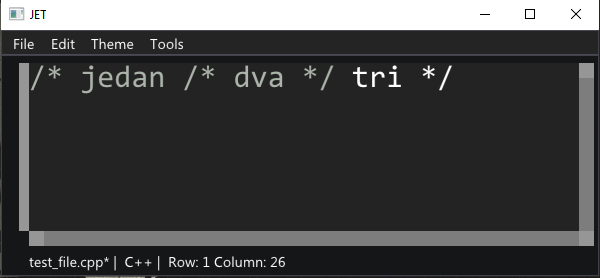
\includegraphics[width=0.8\textwidth]{images/comment_example.png}
	\caption{Пример назначавања коментара}
	\label{fig:comment_example}
\end{figure}
\end{exmp}

\paragraph{}
Треба нагласити да различити токени имају различите приоритете тј.
уколико неки део текста може бити обојен са више боја треба изабрати
само једну. Највиши приоритет имају коментари и ниске,
од претпроцесорских директива једино коментари имају већи приоритет,
док бројеви и кључне речи имају најнижи приоритет. На слици \ref{fig:syntax_priority}
су илустровани приоритети различитих синтаксичких категорија, док је
на сликама \ref{fig:cpp_highlighting}, \ref{fig:c_highlighting},
\ref{fig:cs_highlighting} и \ref{fig:java_highlighting} илустровано редом назначавање програмског кода за језике \begin{latinica}\textit{C++}\end{latinica},
\begin{latinica}\textit{C}\end{latinica}, \begin{latinica}\textit{C\#}\end{latinica}
и \begin{latinica}\textit{Java}\end{latinica}.  Претпроцесорске директиве обојене су
у розе, коментари сивом бојом, ниске су обојене у светло зелено, бројеви жутом
бојом, док су кључне речи обојене наранџасто.

\begin{figure}[!ht]
	\centering
	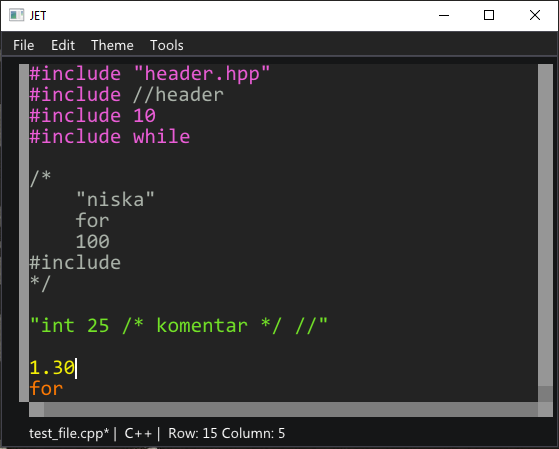
\includegraphics[width=1.0\textwidth]{images/syntax_priority.png}
	\caption{Приказ приоритета између различитих синтаксичких категорија
		\begin{latinica}\textit{C++}\end{latinica}}
	\label{fig:syntax_priority}
\end{figure}

\begin{figure}[!ht]
	\centering
	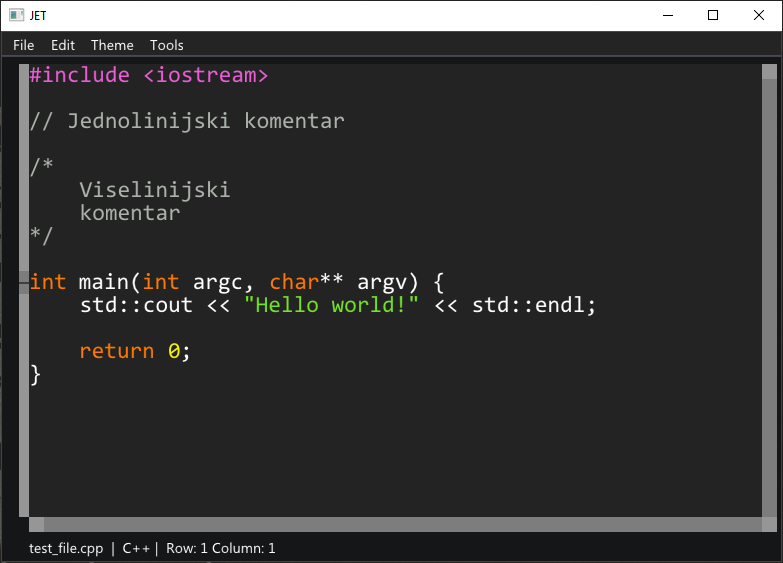
\includegraphics[width=1.0\textwidth]{images/cpp_highlighting.png}
	\caption{Приказ назначавања кода у програмском језику
			\begin{latinica}\textit{C++}\end{latinica}}
	\label{fig:cpp_highlighting}
\end{figure}


\begin{figure}[!ht]
	\centering
	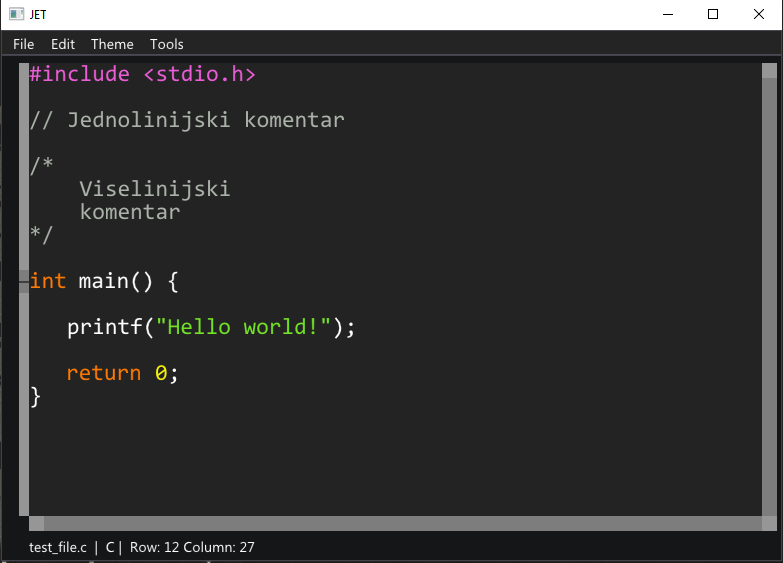
\includegraphics[width=1.0\textwidth]{images/c_highlighting.png}
	\caption{Приказ назначавања кода у програмском језику \begin{latinica}\textit{C}\end{latinica}}
	\label{fig:c_highlighting}
\end{figure}

\begin{figure}[!ht]
	\centering
	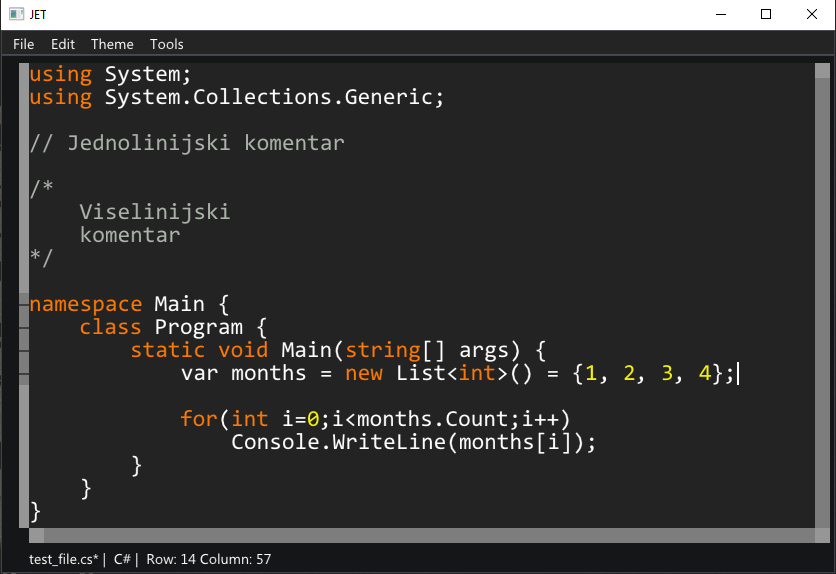
\includegraphics[width=1.0\textwidth]{images/cs_highlighting.png}
	\caption{Приказ назначавања кода у програмском језику
		     \begin{latinica}\textit{C\#}\end{latinica}}
	\label{fig:cs_highlighting}
\end{figure}

\begin{figure}[!ht]
	\centering
	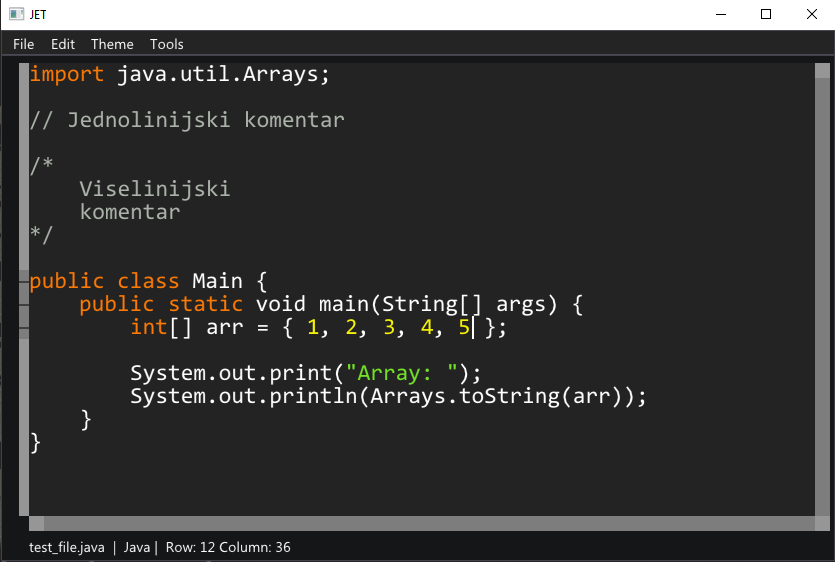
\includegraphics[width=1.0\textwidth]{images/java_highlighting.png}
	\caption{Приказ назначавања кода у програмском језику 
			 \begin{latinica}\textit{Java}\end{latinica}}
	\label{fig:java_highlighting}
\end{figure}

\section{Правоугаоно означавање}

\paragraph{}
У општем случају, означени текст представља непрекидни део текста
између почетне и крајње координате. Међутим, правоугаоно означавање
омогућава да се изабере само онај део текста који је унутар правоугаоника
који чине почетна и крајња координата. 

\begin{figure}[!ht]
	\centering
	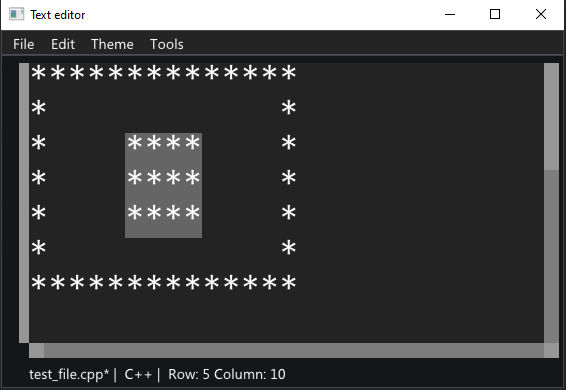
\includegraphics[width=0.8\textwidth]{images/rectangular_selection.png}
	\caption{Приказ правоугаоног означавања}
	\label{fig:rectangular_selection}
\end{figure}

\paragraph{}
То се постиже тако што се додаје индикатор који нам говори да ли
је означавање обично или је правоугаоно. При дохватању означеног
текста, прво се проверава вредност индикатора. Уколико се ради о обичном
означавању, две координате се преводе у индексе и дохвата се текст између
њих. Уколико је се ради о правоугаоном означавању, онда се за сваку линију
почевши од линије почетне координате па до крајње, дохвата текст између колона
почетне и крајње координате. У наредном програмском коду је илустрована ова
функционалност.

\begin{minted}{c++}
std::string Selection::getSelectionText() {
	std::string result;
	TextCoordinates it = m_start.getCoords();
	
	// Dohvata se pokazivač na početnu liniju
	std::string* line = &m_lineBuffer->lineAt(it.m_row-1);
	
	// Iteriranje dok se ne stigne do kraja selekcije
	while (it < m_end.getCoords()) {
		// Ako je kolona van granica, ide se na narednu liniju
		if (it.m_col > line->size() 
		|| (m_rectangular && it.m_col >= m_end.getCoords().m_col)) {
			result += '\n';
			it.m_row += 1;
			it.m_col = m_rectangular ? m_start.getCoords().m_col : 1;
			
			line = &m_lineBuffer->lineAt(it.m_row-1);
		} else {
			if (!line->empty())
			result.push_back(line->at(it.m_col-1));
			
			it.m_col += 1;
		}
	}
	
	return result;
}
\end{minted}

\paragraph{}
Ова функционалност омогућава једноставно дохватање испрекиданих делова
текста као што су колоне у текстуалним табелама као и делове кода без дохватања
карактера за назубљивање. На слици \ref{fig:rectangular_selection} илустровано
је правоугаоно означавање где је означен унутрашњи део звездица.

\section{Подела екрана}

\paragraph{}
Дељење екрана пружа кориснику могућност да има два текстуална поља
којима може прегледати и/или мењати исту датотеку истовремено. Корисник укључује и искључује овај режим преко менија у зависности од потребе. Ова функционалност је корисна у случајевима када текстуална датотека садржи велики број линија и корисник може лакше да прегледа или мења два удаљена места у тексту без сталног пребацивања између њих.

\paragraph{}
Ова функционалност је едитору ЈЕТ остварена тако што
се цртају два објекта класе \begin{latinica}\verb|TextBox|\end{latinica}
који деле показивач на исту табелу делова. Осим што користе исту табелу
делова, све између две инстанце класе \begin{latinica}\verb|TextBox|\end{latinica}  је одвојено.
На слици \ref{fig:split_screen} је илустрована функционалност дељења екрана
за једну датотеку.

\begin{figure}[!ht]
	\centering
	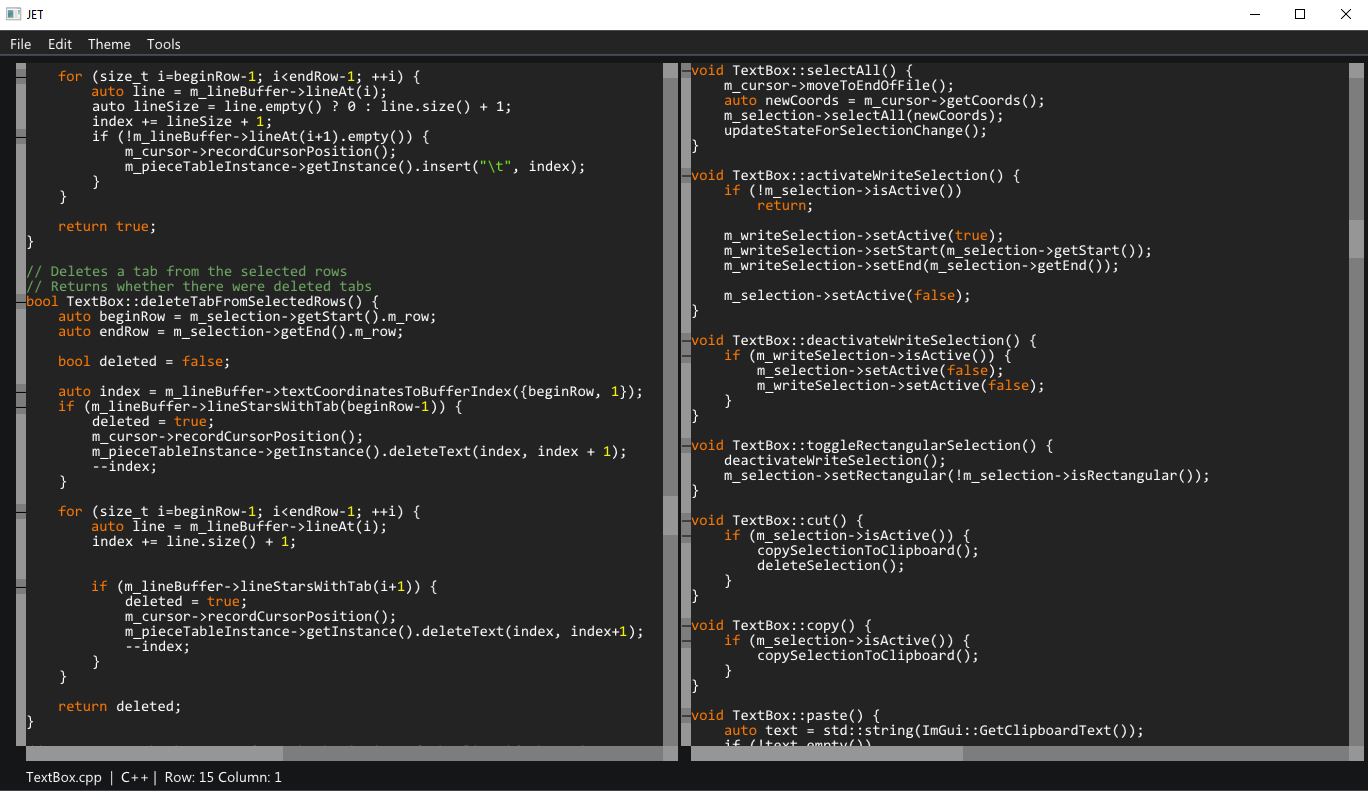
\includegraphics[width=1.0\textwidth]{images/split_screen.png}
	\caption{Приказ поделе екрана}
	\label{fig:split_screen}
\end{figure}


\section{Сужавање простора за измену}

\paragraph{}
Сужавање простора за измену омогућава да се место на коме корисник жели да изврши
измене сузи на неки произвољни опсег текста. Корисник означава неки део текста,
активира ову функционалност из менија и од тада је могуће вршити измене само
унутар означеног дела. Корисник у сваком тренутку може искључити сужавање, враћајући се у уобичајени режим. Ова функционалност може бити корисна у
случајевима када је потребно мењати мање делова кода без нарушавања околне
структуре. Пример овакве измене може бити промена имена функције или променљиве.


\paragraph{}
Ова функционалност је у едитору ЈЕТ имплементирана тако што се при
активирању овог режима памте почетак и крај означеног текста, док у случају ако није означен текст није могуће активирати овај режим. Затим се кретање курсора
и даље означавање текста ограничава на сужени део за измене. То се постиже тако што се за сваку нову позицију курсора врши провера да ли се налази у дозвољеним границама и уколико то није случај поставља се на најближу граничну вредност.  део за измене се, такође, сужава или проширује у зависности од тога
да ли се брише или додаје текст у суженом простору. На слици
\ref{fig:edit_narrowing} илустровано је сужавање дела за измену на име главне
функције.

\begin{figure}[!ht]
	\centering
	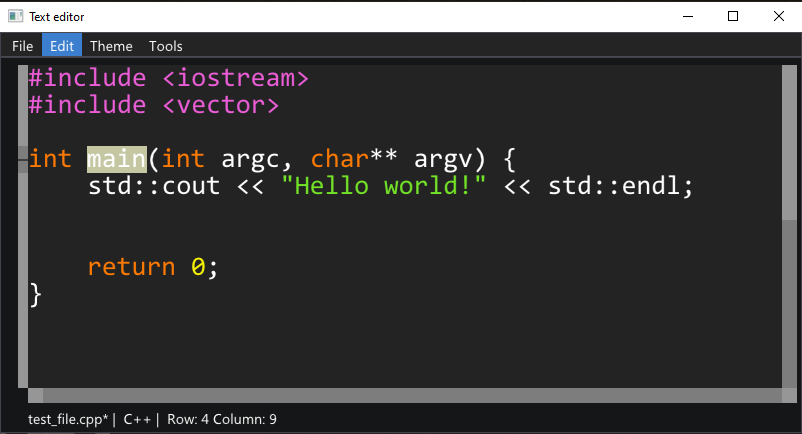
\includegraphics[width=1.0\textwidth]{images/edit_narrowing.png}
	\caption{Приказ сужавања дела за измену}
	\label{fig:edit_narrowing}
\end{figure}


\section{Чување исечака кода}

\paragraph{}
\emph{Исечак кода} (енг. \begin{latinica}\textit{code snippet}\end{latinica})
представља фрагмент кода који се може користити у различитим програмима или
деловима једног програма, исечци се обично чувају у некој датотеци јер представљају корисне делове кода који се могу користити касније и нема потребе
за њиховим поновним писањем. 

\paragraph{}
Чување исечака кода омогућава кориснику да сачува
исечке кода које често користи при писању програмског кода. Сваки исечак састоји се од имена и његовог садржаја. Ова функционалност се користи тако
што корисник отвара мени за исечке у коме му се приказују сви до сада
запамћени исечци. Након одабира жељеног исечка кода корисник може прекопирати његов текст или га обрисати у зависности од потребе. Корисник може додати нови исечак означавањем жељеног текста и одабиром акције додавања исечка из менија, 
уносом имена новог исечка, при чему се, уколико не постоји исечак
са истим именом, он додаје у колекцију. 

\paragraph{}
Описана функционалност је постигнута тако што се исечци чувају у датотекама које се по потреби дохватају и њихов садржај се исписује у менију. Овај мени
је илустрован на слици \ref{fig:code_snippets}.

\begin{figure}[!ht]
	\centering
	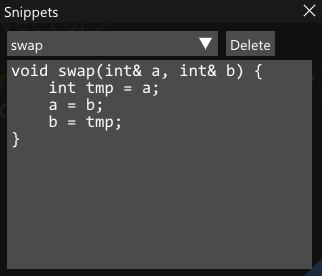
\includegraphics[width=0.5\textwidth]{images/code_snippets.png}
	\caption{Приказ менија за исечке}
	\label{fig:code_snippets}
\end{figure} 

\section{Сакривање блокова}
\paragraph{}
\emph{Сакривање блокова} (енг. \begin{latinica}\textit{code folding}\end{latinica}) је функционалност која кориснику омогућава да сажме 
приказ блока кода у једну линију. Корисник може по потреби да сакрива блокове
кода који му у том тренутку нису релевантни и тако добије бољу прегледност
унутар датотеке. Пре него што наставимо са даљим описом сакривања блокова,
потребно је дефинисати шта представља блок у неком програмском коду.

\paragraph{}
Блок кода је скуп наредби које су логички груписане и чине јединствену целину.
Блокови се најчешће користе за дефинисање функција, наредби контроле тока и петљи.
У већини програмских језика (\begin{latinica}\textit{C++}\end{latinica},
\begin{latinica}\textit{C}\end{latinica}, \begin{latinica}\textit{C\#}\end{latinica},
\begin{latinica}\textit{Java}\end{latinica}) блокови се означавају витичастим заградама, док се код неких, као што је \begin{latinica}\textit{Python}\end{latinica}, они означавају назубљивањем кода. У оквиру едитора \textit{JET} блок се састоји
од почетне и крајње координате као и индикатора да ли је блок сакривен или не.
У наредном програмском коду илустроване су чланске променљиве класе \verb|CodeBlock|.

\begin{minted}{c++}
class CodeBlock {
//...
private:
	TextCoordinates m_start;
	TextCoordinates m_end;
	bool m_folded;
};
\end{minted}

\paragraph{}
У едитору текста \textit{JET}, сакривање блока је имплементирано тако 
што се пролази кроз текст и идентификују се сви блокови. Потом се у првој
линији сваког блока са леве стране додаје дугме за сакривање. Када корисник
кликне на ово дугме, одговарајући блок се сакрива. Сакривени блок се може
поново открити притиском на исто дугме. Пример сакривања блока је илустрован
на слици \ref{fig:code_folding} где је сакривен блок функције \verb|printHelloWorld()|.

\begin{figure}[!ht]
	\centering
	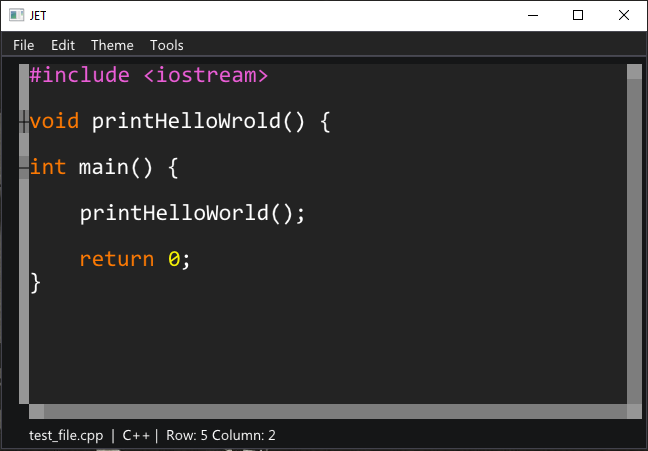
\includegraphics[width=0.8\textwidth]{images/code_folding.png}
	\caption{Пример сакривања блока програмског кода}
	\label{fig:code_folding}
\end{figure} 

\paragraph{}
Евиденција о скривеним линијама кода се чува у низу индикатора који за сваку линију
садржи вредност да ли је скривена или не. Уколико је линија скривена, не исцртава
се у текстуалном пољу, иако и даље постоји унутар текста. 

\paragraph{}
При свакој промени текста потребно је поново идентификовати блокове. Може се десити
да промена текста помери координате постојећих блокова и потребно је да у поновној индентификацији буду препознати као постојећи блокови, а не као нови. То се имплементира тако што се
уз сваку промену текста функцији за ажурирање блокова прослеђује линија на којој је
извршена измена, као број додатих или одузетих линија. Тако да ће функција за
ажурирање блокова, пре него што обради нове блокове, померити координате старих блокова који су захваћени променом текста за одговарајући размак. На крају се за сваки нови
блок, бинарном претрагом, у листи старих блокова тражи одговарајући блок, и уколико постоји, преписује се његово стање у нови. На крају се брише листа старих блокова
и пролсеђује се нова листа. У следећем програмском коду је илустрован рад ове 
функције.

\begin{minted}[tabsize=2]{c++}
void LineBuffer::updateBlocks(int lineSizeDiff, int lineIndex) {
	auto newBlocks = new std::vector<CodeBlock*>();
	std::stack<TextCoordinates> openBrackets;
	auto size = m_lines->size();
	
	if (lineSizeDiff != 0)
	updateFoldedBlocks(lineSizeDiff, lineIndex);
	
	auto oldHidden = m_hidden;
	m_hidden = new std::vector<bool>(size, false);
	delete oldHidden;
	
	for (size_t i=0; i<size; ++i) {
		auto line = m_lines->at(i);
		
		for (size_t j=0; j<line.size(); ++j) {
			if (line[j] == '{') {
  				openBrackets.push(TextCoordinates(i, j+1));
  			} else if (line[j] == '}' && !openBrackets.empty()) {
  				auto openBracket = openBrackets.top();
  				openBrackets.pop();
  				
  				auto closedBracket = TextCoordinates(i, j+1);
  				auto block = new CodeBlock(openBracket, closedBracket);
  				
  				auto index = findBlock(block);
  				
  				if (index != -1 && m_blocks->at(index)->isFolded() == true) {
  					block->setFolded(true);
  					updateHiddenForBlock(block);
  				}
  				
  				newBlocks->push_back(block);
  			}
  		}
  	}
  	
  	auto oldBlocks = m_blocks;
  	m_blocks = newBlocks;
  	
  	for (auto block : *oldBlocks)
  		delete block;
  	delete oldBlocks;
  	
  	std::sort(m_blocks->begin(), m_blocks->end(), 
  			[](CodeBlock* first, CodeBlock* second) { return *first < *second; }
  	);
}

\end{minted}

\paragraph{}
Још једна битна особина код сакривања блокова је угнежђеност. Пошто унутар једног
блока можемо дефинисати прозивољан број блокова, треба приметити да када је
један блок сакривен, сви блокови унутар њега се такође не приказују, без обзира
на то што њихов индикатор сакривености остаје непромењен. Са друге стране, уколико
је блок откривен, сви блокови унутар њега се приказују на основу својих индикатора и правило се рекурзивно примењује на све откривене блокове у њему.  

% ------------------------------------------------------------------------------
% Literatura
% ------------------------------------------------------------------------------
\literatura

% ==============================================================================
% Završni deo teze i prilozi
\backmatter
% ==============================================================================

% ------------------------------------------------------------------------------
% Biografija kandidata
\begin{biografija}
\textbf{Бојан Барџић} је рођен 5. априла 1999. године у Призрену. Основне студије
је завршио на Математичком факултету у Београду, на смеру информатика 2022. године
са просечном оценом 8.64. Тренутно је студент мастер студија на истом факултету.
\end{biografija}
% ------------------------------------------------------------------------------

\end{document} 